\documentclass[12pt,a4paper]{article}
\usepackage[UTF8]{ctex}
\usepackage{amsmath}
\usepackage{amssymb}
\usepackage{graphicx}
\usepackage{hyperref}
\usepackage{geometry}
\usepackage{booktabs}
\usepackage{float}
\usepackage{listings}
\usepackage{xcolor}
\usepackage{multirow}
\usepackage[numbers,sort&compress]{natbib}
\usepackage{algorithm}
\usepackage{algorithmic}

\geometry{left=2.5cm,right=2.5cm,top=2.5cm,bottom=2.5cm}

\title{基于功能脑网络多模版学习的精神疾病辅助诊断算法研究}
\author{}
\date{}

\begin{document}

\maketitle

\newpage

\begin{center}
\Large
\textbf{摘\quad 要}
\end{center}

精神疾病的早期诊断对患者的治疗和生活质量至关重要。然而，传统诊断方法存在局限性，尤其是面对精神疾病的复杂性和多样性。近年来，功能性磁共振成像（fMRI）和深度学习技术的进步为早期诊断带来了新的机遇。

本研究综合运用 fMRI 数据和深度学习技术，特别是多模版功能脑网络分析，旨在提高精神疾病的早期诊断效果。本研究发现，不同脑模版生成的脑网络主要区别在于脑区划分的粒度，这导致了多种视角的信息表达。因此，多模版脑网络学习实际上是一种多视图学习。

以往的研究忽略了不同视图之间的关联和信息冗余。本研究结合多模版功能脑网络分析和深度学习技术提出了一种新的方法，以克服传统方法的局限性。该方法能够利用不同脑模版的多层次信息，结合多视图学习的思想，通过相似性编码器和差异性编码器对视图信息进行解耦和融合，从而实现了对精神疾病的更准确的早期诊断。实验结果表明，该方法在疾病分类任务上取得了显著改进，并有效地捕捉了不同视图之间的关联和信息冗余，提高了信息融合的效果。这一研究成果对精神疾病的早期诊断和治疗具有重要意义，为未来的疾病诊断和治疗提供了新的思路和方法。

\textbf{关键词：}深度学习；多模板；精神疾病；疾病分类

\newpage

\begin{center}
\Large
\textbf{ABSTRACT}
\end{center}

Early diagnosis of mental disorders is crucial for the treatment and quality of life of patients. However, traditional diagnostic methods are limited, especially in the face of the complexity and diversity of mental disorders. In recent years, advances in functional magnetic resonance imaging (fMRI) and deep learning technology have brought new opportunities for early diagnosis.

This study integrates fMRI data and deep learning technology, particularly multi-template functional brain network analysis, aiming to improve the early diagnosis of mental disorders. We found that brain networks generated from different brain templates mainly differ in the granularity of brain region partitioning, leading to information representation from multiple perspectives. Therefore, multi-template brain network learning is essentially a multi-view learning.

Previous studies have overlooked the correlation and information redundancy between different views. We propose a novel method that combines multi-template functional brain network analysis and deep learning technology to overcome the limitations of traditional methods. This method utilizes multi-level information from different brain templates, combines the idea of multi-view learning, and decouples and integrates view information through similarity encoders and discrepancy encoders, thereby achieving more accurate early diagnosis of mental disorders. Experimental results demonstrate that this method significantly improves disease classification tasks and effectively captures the correlation and information redundancy between different views, enhancing the effect of information fusion. This research has important implications for the early diagnosis and treatment of mental disorders, providing new insights and methods for future disease diagnosis and treatment.

\textbf{Key words:} Deep Learning; Multi-template; Mental Disorders; Disease Classification

\newpage

\tableofcontents

\newpage

\section{绪论}

\subsection{研究背景}

\subsubsection{功能性磁共振成像与精神疾病}

功能性磁共振成像（functional Magnetic Resonance Imaging, fMRI）是一种非侵入性的神经影像学技术，能够通过检测血氧水平依赖（Blood Oxygen Level Dependent, BOLD）信号来间接测量大脑活动。静息态 fMRI（resting-state fMRI, rs-fMRI）通过观察受试者在静息状态下的大脑自发活动，可以构建功能连接网络，反映不同脑区之间的功能连接模式。这些连接模式的变化与多种精神疾病密切相关，为疾病的早期诊断提供了重要依据。

精神疾病，如自闭症谱系障碍（Autism Spectrum Disorder, ASD）、精神分裂症、抑郁症等，具有复杂的神经生物学基础。传统的精神疾病诊断主要依赖临床观察和量表评估，存在主观性强、早期诊断困难等问题。因此，基于客观的神经影像学数据进行精神疾病的辅助诊断成为研究热点。

\subsubsection{深度学习方法}

深度学习作为机器学习的一个重要分支，通过构建具有多个隐藏层的神经网络，能够自动学习数据的多层次抽象特征\cite{lecun2015deep}。在医学影像分析领域，深度学习技术已经取得了显著的成果。卷积神经网络（Convolutional Neural Networks, CNN）在图像分类和特征提取方面表现出色；图神经网络（Graph Neural Networks, GNNs）专门用于处理图结构数据，在脑网络分析中具有天然优势；Transformer 模型通过自注意力机制能够捕获长距离依赖关系，在处理序列和图数据时也展现出强大的能力\cite{vaswani2017attention}。

\subsubsection{多模版功能脑网络分析}

不同的脑区划分模板（如 AAL、CC200、CC400 等）由于脑区划分的粒度不同，会生成不同视角的脑网络表示。这些不同模板产生的网络实际上是从不同角度对同一个大脑功能的描述，包含了互补和冗余的信息。多模版分析能够综合利用这些不同粒度的信息，提高疾病诊断的准确性和鲁棒性。

\subsubsection{神经科学与临床诊断的需求}

随着神经影像学技术的不断发展和数据集的日益丰富，如何有效整合多源、多模态的神经影像学数据，构建更加准确和可靠的疾病诊断模型，成为神经科学和临床医学领域迫切需要解决的问题。

\subsubsection{研究意义}

本研究的意义主要体现在以下几个方面：

\begin{enumerate}
\item 理论意义：将多视图学习的思想引入到多模版脑网络分析中，提出了通过相似性和差异性编码器对视图信息进行解耦和融合的新方法，为多视图图数据的融合提供了新的思路。
\item 实践意义：提出的方法在精神疾病辅助诊断任务上取得了良好的效果，为临床诊断提供了新的技术手段。
\item 技术贡献：结合了 Transformer、图神经网络等先进的深度学习技术，构建了一个端到端的诊断模型。
\end{enumerate}

\subsubsection{总结}

综上所述，基于 fMRI 数据和多模版功能脑网络分析，结合深度学习技术进行精神疾病辅助诊断是一个具有重要理论价值和实践意义的研究方向。本研究旨在通过多视图学习的方法，充分利用不同脑模板提供的互补信息，提高疾病诊断的准确性。

\subsection{研究现状}

\subsubsection{基于卷积神经网络（CNN）的方法}

卷积神经网络在医学影像分析中得到了广泛应用。在脑网络分析中，研究者将脑网络的邻接矩阵或连接矩阵视为二维图像，利用 CNN 进行特征提取和分类。这类方法简单直观，能够自动学习脑网络中的局部模式。然而，CNN 主要适用于规则的网格数据，对于图结构数据的处理能力有限，无法充分利用脑网络的拓扑结构信息。

\subsubsection{基于图神经网络（GNN）的方法}

图神经网络专门设计用于处理图结构数据，在脑网络分析中具有天然优势。通过消息传递机制，GNN 能够在节点之间传播信息，学习节点的表示。常见的 GNN 模型包括图卷积网络（Graph Convolutional Network, GCN）\cite{kipf2016semi}、图注意力网络（Graph Attention Network, GAT）\cite{velickovic2017graph}等。这些方法能够有效捕获脑网络的拓扑结构，但通常需要大量的计算资源，且在处理多视图数据时，往往忽略了不同视图之间的关联和冗余信息。

\subsubsection{基于 Transformer 的方法}

Transformer 模型通过自注意力机制能够捕获长距离依赖关系，在处理序列和图数据时展现出强大的能力。在脑网络分析中，有研究者将脑网络中的节点或边序列化，然后使用 Transformer 进行处理。也有研究将 Transformer 与图神经网络结合，利用 Transformer 的注意力机制来增强图神经网络的表达能力。然而，这些方法在处理多视图数据时，往往缺乏对视图间相似性和差异性的显式建模。

\subsubsection{其他深度学习方法}

除了上述方法外，还有研究者采用自编码器、变分自编码器等无监督学习方法对脑网络进行特征提取，然后使用传统的机器学习方法进行分类。也有研究采用集成学习方法，将多个模型的结果进行融合。这些方法各有优势，但在多视图信息的有效融合方面仍有改进空间。

\subsubsection{总结}

现有的方法主要存在以下问题：

\begin{enumerate}
\item 大多数方法只关注单个模板或视图，忽略了多模板提供的互补信息。
\item 即使使用多个模板，也往往只是简单地拼接特征或独立处理，没有充分考虑不同视图之间的关联和冗余。
\item 缺乏对视图间相似性和差异性的显式建模，难以实现信息的有效融合。
\end{enumerate}

因此，本研究旨在提出一种能够有效融合多视图信息的方法，通过显式建模视图间的相似性和差异性，实现更好的信息融合效果。

\subsection{本文的研究内容和技术路线}

\subsubsection{本文的研究内容}

本文的主要研究内容包括：

\begin{enumerate}
\item 分析不同脑模板生成的脑网络的特点，理解多模版脑网络学习的本质。
\item 设计并实现基于 Transformer 的编码器，用于从单个脑模板中提取特征。
\item 提出多视图融合方法，通过相似性编码器和差异性编码器对视图信息进行解耦和融合。
\item 在 ABIDE 数据集上进行实验，验证所提方法的有效性。
\item 分析实验结果，探讨不同组件对模型性能的贡献。
\end{enumerate}

\subsubsection{本文研究路线}

本文的技术路线如下：

\begin{enumerate}
\item 数据预处理：对 ABIDE 数据集中的 rs-fMRI 数据进行预处理，构建功能连接网络。
\item 编码器设计：设计基于 Transformer 的编码器，用于从不同模板的脑网络中提取特征。
\item 多视图融合：设计相似性编码器和差异性编码器，实现多视图信息的解耦和融合。
\item 模型训练：设计损失函数，包括分类损失、相似性损失和差异性损失，对模型进行端到端的训练。
\item 实验评估：在 ABIDE 数据集上进行十折交叉验证，评估模型的性能。
\item 结果分析：分析实验结果，探讨模型的有效性和不同组件的作用。
\end{enumerate}

\section{基础理论介绍}

\subsection{人工智能理论}

人工智能（Artificial Intelligence, AI）旨在使机器能够模拟人类的智能行为，包括学习、推理、感知等。机器学习（Machine Learning, ML）是人工智能的一个重要分支，通过从数据中学习模式和规律，使机器能够自动完成特定任务。深度学习（Deep Learning, DL）是机器学习的一个子领域，通过构建具有多个隐藏层的神经网络，能够自动学习数据的多层次抽象特征。

在本研究中，深度学习技术被应用于精神疾病的辅助诊断任务。通过构建多层神经网络模型，本研究能够从功能脑网络数据中自动学习疾病相关的特征模式，避免了传统方法中需要手工设计特征的局限性。实验结果表明，基于深度学习的多模板融合方法在 ABIDE 数据集上取得了 0.692385 的准确率，证明了深度学习在脑网络分析中的有效性。

\subsection{模型理论}

\subsubsection{卷积神经网络（Convolutional Neural Networks, CNN）}

卷积神经网络是一种专门用于处理具有网格拓扑结构数据的深度学习模型。CNN 的核心思想是通过卷积操作和池化操作来提取数据的局部特征，并通过多层网络的堆叠来学习数据的层次化表示。在图像处理任务中，CNN 取得了革命性的成果。

CNN 的主要组件包括：
\begin{itemize}
\item 卷积层：通过卷积核在输入数据上进行滑动窗口操作，提取局部特征。
\item 池化层：对特征图进行下采样，减少参数数量，提高模型的鲁棒性。
\item 全连接层：将提取的特征映射到输出空间。
\end{itemize}

在本研究中，CNN 被应用于 BrainNetCNN（E2E）编码器的设计中。该编码器使用边到边（Edge-to-Edge, E2E）、边到节点（Edge-to-Node, E2N）和节点到图（Node-to-Graph, N2G）的卷积操作来提取脑网络连接矩阵中的局部模式。虽然最终实验表明 SimpleTransformer 编码器在准确率和计算效率方面表现更优（ACC = 0.677273，训练时间 3.49 秒），但 CNN 方法（ACC = 0.642881，训练时间 71.13 秒）的探索为理解不同特征提取策略的优劣提供了重要参考。

\subsubsection{Transformer}

Transformer 是一种基于自注意力机制的深度学习模型，最初用于序列到序列的任务\cite{vaswani2017attention}。与循环神经网络和卷积神经网络不同，Transformer 完全依赖于注意力机制来捕获序列中的依赖关系，使得模型能够并行处理序列中的所有位置。

Transformer 的核心组件包括：

\paragraph{自注意力机制}
自注意力机制（Self-Attention）允许模型在计算每个位置的表示时，直接关注到序列中的所有其他位置。对于输入序列 $X = [x_1, x_2, \ldots, x_n]$，自注意力机制通过以下步骤计算：

首先，将输入转换为查询（Query, Q）、键（Key, K）和值（Value, V）三个矩阵：
\begin{equation}
Q = XW_Q, \quad K = XW_K, \quad V = XW_V
\end{equation}

其中 $W_Q$、$W_K$、$W_V$ 是可学习的权重矩阵。

然后，计算注意力分数：
\begin{equation}
\text{Attention}(Q, K, V) = \text{softmax}\left(\frac{QK^T}{\sqrt{d_k}}\right)V
\end{equation}

其中 $d_k$ 是键向量的维度，$\sqrt{d_k}$ 用于缩放，避免点积值过大导致梯度消失。

多头注意力（Multi-Head Attention）通过并行运行多个注意力机制来捕获不同类型的关系：
\begin{equation}
\text{MultiHead}(Q, K, V) = \text{Concat}(\text{head}_1, \ldots, \text{head}_h)W^O
\end{equation}

其中每个注意力头定义为：
\begin{equation}
\text{head}_i = \text{Attention}(QW_i^Q, KW_i^K, VW_i^V)
\end{equation}

\paragraph{位置编码}
由于 Transformer 不包含循环或卷积结构，需要显式地注入位置信息。位置编码通过以下公式添加到输入嵌入中：
\begin{equation}
PE_{(pos, 2i)} = \sin\left(\frac{pos}{10000^{2i/d_{model}}}\right)
\end{equation}

\begin{equation}
PE_{(pos, 2i+1)} = \cos\left(\frac{pos}{10000^{2i/d_{model}}}\right)
\end{equation}

其中 $pos$ 是位置，$i$ 是维度索引，$d_{model}$ 是模型维度。

\paragraph{前馈神经网络}
前馈神经网络（Feed-Forward Network, FFN）对注意力输出进行非线性变换：
\begin{equation}
\text{FFN}(x) = \max(0, xW_1 + b_1)W_2 + b_2
\end{equation}

通常使用 ReLU 激活函数。

\paragraph{残差连接和层归一化}
Transformer 在每个子层周围使用残差连接和层归一化：
\begin{equation}
\text{LayerNorm}(x + \text{Sublayer}(x))
\end{equation}

这有助于训练深层网络，缓解梯度消失问题。

在本研究中，Transformer 架构被应用于 SimpleTransformer 编码器的设计中，用于从单个脑模板的连接矩阵中提取特征。具体而言，本研究将脑网络的连接矩阵重塑为序列形式，通过 Transformer 编码器的自注意力机制捕获不同脑区之间的长距离依赖关系。实验结果表明，SimpleTransformer 编码器在 CC400 模板上取得了 0.677273 的准确率，优于 CNN 和 GNN 方法，证明了 Transformer 在处理脑网络数据时的有效性。此外，Transformer 的并行计算特性使得模型训练时间仅为 3.49 秒，显著优于其他方法。在多模板融合阶段，本研究进一步使用 Transformer 编码器对来自不同模板的特征进行融合和增强，通过自注意力机制捕获不同视图之间的关联关系，最终实现了 0.692385 的准确率，验证了 Transformer 在多视图学习中的优势。

\subsubsection{图神经网络（Graph Neural Networks, GNNs）}

图神经网络是一类专门用于处理图结构数据的深度学习模型。在脑网络分析中，脑网络可以自然地表示为图结构，其中节点表示脑区，边表示脑区之间的连接。

图神经网络的核心思想是通过消息传递机制，在节点之间传播信息，从而学习节点的表示。假设图 $G = (V, E)$，其中 $V$ 是节点集合，$E$ 是边集合。对于节点 $v$，其邻居集合记为 $\mathcal{N}(v)$。

\paragraph{图卷积网络（GCN）}
图卷积网络通过聚合邻居节点的特征来更新节点表示。对于节点 $v$，其表示在第 $l$ 层的更新公式为：

\begin{equation}
h_v^{(l+1)} = \sigma\left(W^{(l)} \sum_{u \in \mathcal{N}(v) \cup \{v\}} \frac{1}{\sqrt{|\mathcal{N}(u)||\mathcal{N}(v)|}} h_u^{(l)}\right)
\end{equation}

其中 $h_v^{(l)}$ 是节点 $v$ 在第 $l$ 层的表示，$W^{(l)}$ 是可学习的权重矩阵，$\sigma$ 是激活函数（如 ReLU）。

使用矩阵形式，可以表示为：
\begin{equation}
H^{(l+1)} = \sigma\left(\tilde{D}^{-\frac{1}{2}}\tilde{A}\tilde{D}^{-\frac{1}{2}} H^{(l)} W^{(l)}\right)
\end{equation}

其中 $\tilde{A} = A + I$ 是添加自连接的邻接矩阵，$\tilde{D}$ 是度矩阵，$H^{(l)}$ 是节点特征矩阵。

\paragraph{图注意力网络（GAT）}
图注意力网络使用注意力机制来确定邻居节点的重要性。对于节点 $v$，其表示更新为：

\begin{equation}
h_v^{(l+1)} = \sigma\left(\sum_{u \in \mathcal{N}(v) \cup \{v\}} \alpha_{vu}^{(l)} W^{(l)} h_u^{(l)}\right)
\end{equation}

其中注意力权重 $\alpha_{vu}^{(l)}$ 通过以下方式计算：

\begin{equation}
\alpha_{vu}^{(l)} = \frac{\exp\left(\text{LeakyReLU}\left(a^T [W^{(l)} h_v^{(l)} || W^{(l)} h_u^{(l)}]\right)\right)}{\sum_{w \in \mathcal{N}(v) \cup \{v\}} \exp\left(\text{LeakyReLU}\left(a^T [W^{(l)} h_v^{(l)} || W^{(l)} h_w^{(l)}]\right)\right)}
\end{equation}

其中 $a$ 是注意力机制的参数向量，$||$ 表示拼接操作。

\paragraph{GraphSAGE}
GraphSAGE（Graph Sample and Aggregate）通过采样和聚合邻居节点来学习节点表示，适用于大规模图。其更新公式为：

\begin{equation}
h_v^{(l+1)} = \sigma\left(W^{(l)} \cdot \text{CONCAT}(h_v^{(l)}, \text{AGG}(\{h_u^{(l-1)}, \forall u \in \mathcal{N}(v)\}))\right)
\end{equation}

其中 $\text{AGG}$ 是聚合函数，可以是均值、最大值或 LSTM 等。

在本研究中，图神经网络的思想被应用于 SGFormer 编码器的设计中。SGFormer 结合了图卷积操作和 Transformer 的自注意力机制，理论上能够更好地利用脑网络的拓扑结构信息。然而，实验结果表明，SGFormer 在 CC400 模板上的准确率仅为 0.536181，且训练时间最长（89.25 秒），这可能与其复杂的模型结构和较高的计算复杂度有关。虽然 GNN 方法在本研究中未取得最佳性能，但其对图结构数据的处理思想为后续研究提供了重要参考。值得注意的是，本研究中的 SimpleTransformer 编码器虽然主要基于 Transformer 架构，但其处理脑网络连接矩阵的方式实际上也体现了图数据的序列化表示思想，这反映了不同深度学习范式之间的相互借鉴和融合。

\subsection{实验方法理论}

\subsubsection{交叉验证}

交叉验证是一种评估模型性能的统计方法\cite{kohavi1995study}，通过将数据集划分为多个子集，轮流使用其中的一个子集作为测试集，其余子集作为训练集，从而获得多个性能评估结果。十折交叉验证是最常用的交叉验证方法之一，将数据集划分为 10 个子集，进行 10 次训练和测试，最后取平均结果作为模型的性能评估。

在本研究中，十折交叉验证被用于评估所有模型的性能。具体而言，将包含 871 名受试者的 ABIDE 数据集随机划分为 10 个子集，每次使用 9 个子集作为训练集（约 784 个样本），1 个子集作为测试集（约 87 个样本），重复 10 次实验后取平均值作为最终性能指标。这种评估方法能够有效减少因数据划分带来的随机性影响，提供更加可靠和稳定的性能评估结果。实验结果表明，MultiModalBrainModel 在十折交叉验证中取得了平均准确率 0.692385、召回率 0.680739、F1 评分 0.671735 和 AUC 0.729583 的性能，证明了模型具有良好的泛化能力。

\subsubsection{超参数（Hyperparameters）和参数（Parameters）}

在机器学习中，参数是模型在学习过程中自动调整的变量，如神经网络中的权重和偏置。而超参数是在训练开始之前需要人为设定的参数，如学习率、批次大小、网络层数等。超参数的选择对模型的性能有很大影响，通常需要通过网格搜索、随机搜索等方法来确定最优的超参数组合。

在本研究中，通过实验确定了以下关键超参数：模型维度（$d_{model}$）为 32，特征维度（$d_{feature}$）为 2，融合维度（$d_{fusion}$）为 16，注意力头数为 2，Transformer 层数为 1（特征提取阶段）和 2（融合阶段），Dropout 率为 0.25（特征提取）和 0.5（融合），学习率为 0.001，批次大小为 32，训练轮数为 100。这些超参数的选择对模型性能有重要影响，例如，实验发现较小的模型维度（32）能够在保持性能的同时降低计算复杂度，而适当的 Dropout 率能够有效防止过拟合，提高模型的泛化能力。

\subsubsection{反向传播算法（Backpropagation Algorithm）}

反向传播算法是训练多层神经网络的核心算法\cite{rumelhart1986learning}。它通过计算损失函数对模型参数的梯度，然后使用梯度下降等方法更新参数，使模型能够最小化损失函数。反向传播算法利用链式法则，从输出层向输入层逐层传播梯度信息。

在本研究中，反向传播算法被用于训练 MultiModalBrainModel。模型使用 Adam 优化器，通过反向传播算法计算总损失（包括分类损失、相似性损失和差异性损失）对模型参数的梯度，然后更新参数以最小化损失函数。实验结果表明，通过反向传播算法训练的模型能够有效学习脑网络中的疾病相关模式，最终在测试集上取得了良好的分类性能。此外，本研究还使用了学习率调度策略（如 StepLR 或 CosineAnnealingLR），通过动态调整学习率来优化训练过程，这进一步体现了反向传播算法在深度学习训练中的核心作用。

\subsection{评价指标}

\subsubsection{准确率（ACC）}

准确率是最常用的分类性能评估指标，定义为正确分类的样本数占总样本数的比例：

\begin{equation}
ACC = \frac{TP + TN}{TP + TN + FP + FN}
\end{equation}

其中，TP（True Positive）表示真正例，TN（True Negative）表示真负例，FP（False Positive）表示假正例，FN（False Negative）表示假负例。

在本研究中，准确率被用作评估模型性能的主要指标之一。实验结果表明，MultiModalBrainModel 在 ABIDE 数据集上取得了 0.692385 的准确率，相比于单一模板的 SimpleTransformer 方法（CC400 模板：0.686507，AAL 模板：0.622309）有所提升，证明了多视图融合策略的有效性。准确率指标能够直观地反映模型整体分类的正确性，对于二分类任务（ASD vs. 正常对照）具有重要的参考价值。

\subsubsection{召回率（Recall）}

召回率（也称为敏感性）定义为真正例占实际正例的比例：

\begin{equation}
Recall = \frac{TP}{TP + FN}
\end{equation}

召回率反映了模型对正例的识别能力。

在本研究中，召回率被用于评估模型对 ASD 患者的识别能力。实验结果表明，MultiModalBrainModel 的召回率为 0.680739，表明模型能够识别出约 68\% 的 ASD 患者。在医学诊断任务中，召回率是一个重要的指标，因为漏诊（假阴性）可能比误诊（假阳性）带来更严重的后果。较高的召回率表明模型能够有效识别出大部分 ASD 患者，这对于早期诊断和治疗具有重要意义。

\subsubsection{F1 评分}

F1 评分是精确率（Precision）和召回率的调和平均数：

\begin{equation}
F1 = \frac{2 \times Precision \times Recall}{Precision + Recall} = \frac{2TP}{2TP + FP + FN}
\end{equation}

F1 评分综合考虑了精确率和召回率，是一个平衡的评估指标。

在本研究中，F1 评分被用于综合评估模型的分类性能。实验结果表明，MultiModalBrainModel 的 F1 评分为 0.671735，相比于单一模板方法（CC400：0.681376，AAL：0.626127）表现稳定。F1 评分能够平衡精确率和召回率，避免模型过度偏向某一指标。在医学诊断任务中，F1 评分提供了一个综合的性能评估，有助于全面理解模型的诊断能力。

\subsubsection{曲线下面积（AUC）}

AUC（Area Under the Curve）是 ROC 曲线（Receiver Operating Characteristic curve）下的面积。ROC 曲线以假正例率（False Positive Rate, FPR）为横轴，真正例率（True Positive Rate, TPR）为纵轴。AUC 值越大，说明模型的分类性能越好。AUC 值在 0.5 到 1.0 之间，其中 0.5 表示随机分类，1.0 表示完美分类。

在本研究中，AUC 被用于评估模型在不同分类阈值下的整体性能。实验结果表明，MultiModalBrainModel 的 AUC 为 0.729583，虽然略低于单一 CC400 模板的 SimpleTransformer 方法（0.756921），但显著高于 AAL 模板方法（0.688950）。AUC 指标不依赖于特定的分类阈值，能够全面评估模型的分类能力。在医学诊断中，AUC 值反映了模型区分 ASD 患者和正常对照的能力，0.729583 的 AUC 值表明模型具有中等偏上的诊断能力，为临床辅助诊断提供了有价值的参考。

\section{基于多模板的疾病诊断算法研究与实验}

\subsection{数据集介绍}

\subsubsection{ABIDE（Autism Brain Imaging Data Exchange）}

ABIDE 是一个公共的自闭症研究数据库\cite{dimartino2014autism}，汇集了来自 17 个不同采集点的 1112 名受试者的 rs-fMRI 和表型数据。该数据集包含了丰富的自闭症谱系障碍（ASD）患者与健康对照组（Typically Developing, TD）的脑成像数据。在本研究中，使用 Connectome Computing System 对图像进行预处理，预处理步骤包括切片定时校正、运动校正和体素强度归一化等。最终共纳入 871 名优质受试者，包括 403 名 ASD 患者（女性 54 名，男性 349 名，年龄 17.07±7.96 岁，范围 7-58 岁）和 468 名正常对照（女性 90 名，男性 378 名，年龄 16.84±7.24 岁，范围 6-56 岁）。

\subsubsection{脑区划分模板}

在脑网络研究中，常用的脑区划分模板有多个，包括 AAL（Automated Anatomical Labeling）、CC200（Craddock 200）、CC400（Craddock 400）、DOS160（Dosenbach 160）、EZ（Eickhoff-Zilles）、HO（Harvard-Oxford）和 TT（Talairach-Tournoux）等。

\begin{itemize}
\item \textbf{AAL 模板}：一种基于结构的脑区划分方法，将脑分为 116 个区域\cite{tzourio2002automated}。该模板广泛应用于功能和结构连接研究，基于结构 MRI 数据，提供标准化的脑区划分。

\item \textbf{CC200 模板}：一种基于功能的脑区划分方法，通过聚类分析将脑分为 200 个功能连接区域\cite{craddock2012whole}。该模板通过聚类算法基于 rs-fMRI 数据生成，强调功能连接的同质性。

\item \textbf{CC400 模板}：CC200 的扩展版本\cite{craddock2012whole}，通过更细粒度的聚类将脑分为 400 个功能连接区域，提供了更高分辨率的功能连接划分。

\item \textbf{DOS160 模板}：基于 Dosenbach 等人提出的一种包含 160 个 ROI 的功能连接模板\cite{dosenbach2010prediction}，主要用于任务态和静息态功能连接研究。

\item \textbf{EZ 模板}：基于 Eickhoff 和 Zilles 提出的脑区划分方法\cite{eickhoff2005new}，本研究中脑区数量为 116。该模板提供高分辨率的解剖学细节。

\item \textbf{HO 模板}：由 Harvard 大学和 Oxford 大学联合开发，基于高分辨率的结构 MRI 数据，将脑分为 96 个区域\cite{desikan2006automated}。

\item \textbf{TT 模板}：基于 Talairach 和 Tournoux 的脑区坐标系统\cite{lancaster2007bias}，本研究中脑区数量为 97。该模板是经典的脑区坐标系统，适用于标准化的脑成像研究。
\end{itemize}

不同模板生成的脑网络主要区别在于脑区划分的粒度不同，导致在不同脑模板上有多种视角的信息表达，因此多模版脑网络学习实际上是一种多视图学习。

数据表示为反映脑区之间连通性的图。例如，对于 CC200 模板，有 200 个脑区，图的大小为 (200, 200)，整个数据集存放的矩阵为 (871, 200, 200)。

\paragraph{数据预处理流程}
在使用 ABIDE 数据集之前，需要进行以下预处理步骤：

\begin{enumerate}
\item \textbf{数据加载}：从 MAT 文件中加载脑网络连接矩阵，连接强度通过 Pearson 相关系数计算得到。

\item \textbf{异常值处理}：
\begin{itemize}
\item NaN 值处理：将连接矩阵中的 NaN 值替换为 0，表示该连接不存在或无法计算。
\item Inf 值处理：将连接矩阵中的无穷大值（Inf）替换为 1，表示强连接。
\item 数据范围检查：确保连接值在合理范围内（通常在 $[-1, 1]$ 之间，对于相关系数）。
\end{itemize}

\item \textbf{数据归一化}（可选）：
\begin{itemize}
\item Z-score 标准化：$X_{norm} = \frac{X - \mu}{\sigma}$，其中 $\mu$ 和 $\sigma$ 分别为均值和标准差。
\item Min-Max 归一化：$X_{norm} = \frac{X - X_{min}}{X_{max} - X_{min}}$。
\item 本研究主要使用原始相关系数值，因为其在生物学上具有明确的解释意义。
\end{itemize}

\item \textbf{数据划分}：
\begin{itemize}
\item 按照十折交叉验证的要求，将数据集随机划分为 10 个子集。
\item 每次实验使用 9 个子集作为训练集，1 个子集作为测试集。
\item 确保每个子集中 ASD 和正常对照的样本比例与整体数据集保持一致。
\end{itemize}
\end{enumerate}

\paragraph{数据可视化}
图 \ref{fig:cc200} 和图 \ref{fig:ez} 分别展示了一个典型病人的 CC200 和 EZ 模板连接矩阵热图。从图中可以看出，不同脑区之间的连接强度存在明显的差异，形成了特定的连接模式。这种连接模式可能反映了大脑的功能组织，对于疾病诊断具有重要价值。

不同脑模板由于脑区划分的粒度不同，生成的热图表现出不同的特征。CC200 模板将脑分为 200 个功能连接区域，提供了中等粒度的功能划分；而 EZ 模板将脑分为 116 个区域，更注重解剖学细节和结构划分。这种不同的划分方式使得同一大脑的功能连接网络在不同模板下呈现出不同的表示视角，从而包含了互补的信息。多模板分析正是利用这种多视角的信息表达，通过整合不同粒度的特征来提高疾病诊断的准确性和鲁棒性。

\begin{figure}[H]
\centering
\includegraphics[width=0.6\textwidth]{../png/cc200.png}
\caption{一个病人的 CC200 热图，展示了不同脑区之间的功能连接强度}
\label{fig:cc200}
\end{figure}

\begin{figure}[H]
\centering
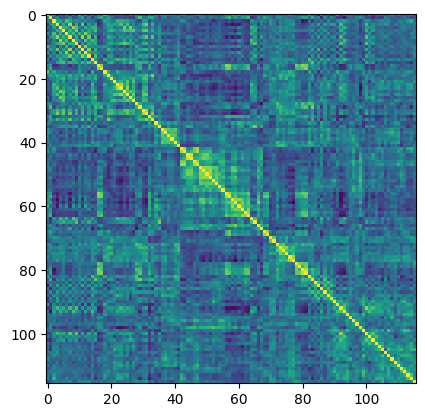
\includegraphics[width=0.6\textwidth]{../png/ez.png}
\caption{一个病人的 EZ 热图，展示了不同脑区之间的功能连接强度}
\label{fig:ez}
\end{figure}

\paragraph{数据统计信息}
表 \ref{tab:data_stats} 展示了 ABIDE 数据集的详细统计信息。

\begin{table}[H]
\centering
\caption{ABIDE 数据集统计信息}
\label{tab:data_stats}
\begin{tabular}{lcc}
\toprule
统计指标 & ASD 患者 & 正常对照 \\
\midrule
样本数量 & 403 & 468 \\
男性 & 349 & 378 \\
女性 & 54 & 90 \\
年龄（岁，均值±标准差） & 17.07±7.96 & 16.84±7.24 \\
年龄范围（岁） & 7-58 & 6-56 \\
\bottomrule
\end{tabular}
\end{table}

\subsection{实验环境}

\subsubsection{硬件环境}

本研究的实验主要在以下硬件环境下进行：
\begin{itemize}
\item GPU：NVIDIA RTX 4080 Laptop（12GB 显存）
\item CPU：Intel Core i9-13900HX 处理器
\item 内存：DDR4 64GB
\end{itemize}

实验中的计算时间均基于上述硬件环境测量。

\subsubsection{软件环境}

实验使用的软件环境包括：
\begin{itemize}
\item 操作系统：Windows 11（在 WSL、Ubuntu、macOS 上都测试可以运行）
\item Python：Python 3.9+ 版本（通过 uv 管理）
\item 深度学习框架：PyTorch $\geq$ 2.8.0
\item 数据处理库：NumPy 1.23.5、SciPy 1.10.1、Pandas 1.5.1
\item 机器学习工具：scikit-learn 1.1.3
\item 图神经网络库：torch-geometric 1.7.2、torch-sparse $\geq$ 0.6.18、torch-scatter $\geq$ 2.1.2
\item 可视化库：Matplotlib 3.6.2
\item 其他依赖库：详见 pyproject.toml 和 requirements.txt 配置文件
\end{itemize}

所有依赖包通过 uv 包管理器进行管理，确保实验环境的一致性和可复现性。

\subsubsection{实验方法}

本研究采用十折交叉验证方法评估模型性能。具体流程如下：
\begin{enumerate}
\item 将数据集随机划分为 10 个子集
\item 依次使用 9 个子集作为训练集，1 个子集作为测试集
\item 重复训练和测试 10 次，每次使用不同的测试集
\item 计算 10 次实验结果的平均值和标准差作为最终性能指标
\end{enumerate}

为了确保实验的可重复性，所有实验均设置了随机种子（seed = 123），并使用相同的随机划分策略。

\subsection{基于单模板的模型特征提取编码器算法研究}

为了高效地从原始脑模板数据中提取特征，本研究实验了三个编码器：基于边卷积的 E2E 模型（BrainNetCNN）、从超图理论获得灵感的 SimpleTransformer 模型（Transformer 编码器），以及融合了图神经网络（GNN）和 Transformer 的 SGFormer 编码器。本节详细介绍这三种编码器的设计和实现。

\subsubsection{Transformer 编码器}

SimpleTransformer 编码器是基于 Transformer 架构设计的特征提取模型。该模型从超图理论获得灵感\cite{feng2019hypergraph}，能够有效捕获脑网络中节点间的长距离依赖关系。

模型的主要组件包括：
\begin{itemize}
\item \textbf{输入层}：将原始脑网络特征（连接矩阵）转换为模型维度，并通过批归一化层进行归一化处理。
\item \textbf{Transformer 编码器层}：使用多头自注意力机制捕获节点间的复杂关系。模型采用单层 Transformer 编码器，包含 2 个注意力头。
\item \textbf{输出层}：对 Transformer 编码器的输出进行聚合（平均池化），然后通过全连接层输出特征向量。
\end{itemize}

SimpleTransformer 模型的关键优势在于其能够并行处理所有节点，并且通过自注意力机制捕获全局依赖关系，这对于处理脑网络的拓扑结构非常重要。

算法的伪代码描述如下：

\begin{algorithm}[H]
\caption{SimpleTransformerModel}
\begin{algorithmic}[1]
\REQUIRE 脑网络连接矩阵 $X \in \mathbb{R}^{N \times N}$，模型维度 $d_{model}$，特征维度 $d_{feature}$，注意力头数 $n_{head}$，层数 $n_{layer}$
\ENSURE 特征向量 $f \in \mathbb{R}^{d_{feature}}$
\STATE 初始化模型参数：$input\_dim = N^2$, $model\_dim$, $feature\_dim$, $num\_heads$, $num\_layers$, $dropout$
\STATE 定义输入全连接层：$input\_fc: \mathbb{R}^{N^2} \rightarrow \mathbb{R}^{d_{model}}$
\STATE 定义输入批归一化层：$input\_bn$
\STATE 定义 Transformer 编码器层：$transformer$（包含 $num\_layers$ 层，每层 $num\_heads$ 个注意力头）
\STATE 定义输出批归一化层：$output\_bn$
\STATE 定义输出全连接层：$output\_fc: \mathbb{R}^{d_{model}} \rightarrow \mathbb{R}^{d_{feature}}$
\STATE // 前向传播
\STATE $x \leftarrow \text{Flatten}(X)$ \quad // 将连接矩阵展平为 $[N^2]$
\STATE $x \leftarrow \text{Reshape}(x, (N, N))$ \quad // 重塑为序列形式 $[N, N]$
\STATE $h \leftarrow input\_fc(x)$ \quad // $[N, d_{model}]$
\STATE $h \leftarrow input\_bn(h)$ \quad // 批归一化
\STATE $h \leftarrow h.permute(1, 0, 2)$ \quad // 调整为 $(seq\_len, batch, d_{model})$ 格式
\STATE $h \leftarrow transformer(h)$ \quad // Transformer 编码，多头自注意力 + FFN
\STATE $h_{graph} \leftarrow h.mean(dim=0)$ \quad // 序列维度平均池化，$[d_{model}]$
\STATE $h_{graph} \leftarrow output\_bn(h_{graph})$ \quad // 输出批归一化
\STATE $f \leftarrow output\_fc(h_{graph})$ \quad // $[d_{feature}]$
\RETURN $f$
\end{algorithmic}
\end{algorithm}

\textbf{复杂度分析：}
SimpleTransformer 的时间复杂度主要由 Transformer 编码器的自注意力机制决定。对于输入序列长度为 $N$，模型维度为 $d_{model}$，注意力头数为 $n_{head}$，层数为 $n_{layer}$ 的模型：
\begin{itemize}
\item \textbf{时间复杂度}：$O(n_{layer} \cdot (N^2 \cdot d_{model} + N \cdot d_{model}^2))$，其中第一项为自注意力机制的计算复杂度，第二项为前馈网络的计算复杂度。
\item \textbf{空间复杂度}：$O(N^2 + d_{model}^2)$，主要由注意力矩阵和模型参数决定。
\end{itemize}

相比于 CNN 方法，SimpleTransformer 虽然具有更高的理论复杂度，但由于 Transformer 的并行计算特性，在实际训练中能够充分利用 GPU 的并行能力，从而获得更高的计算效率。

\subsubsection{SGFormer 编码器}

SGFormer（Semi-supervised Graph Transformer）是一个融合了图神经网络和 Transformer 的混合模型\cite{thomas2021sgformer}。该模型结合了 GNN 的图结构处理能力和 Transformer 的注意力机制。

SGFormer 的主要特点：
\begin{itemize}
\item 使用图卷积操作捕获局部邻居信息
\item 通过 Transformer 的自注意力机制捕获全局依赖关系
\item 结合了图结构信息和序列建模能力
\end{itemize}

算法的伪代码描述如下：

\begin{algorithm}[H]
\caption{SGFormer}
\begin{algorithmic}[1]
\REQUIRE 脑网络连接矩阵 $X \in \mathbb{R}^{N \times N}$，邻接矩阵 $A \in \mathbb{R}^{N \times N}$
\ENSURE 分类输出 $y$
\STATE 初始化模型参数：节点数 $N$，特征维度 $d$，注意力头数 $n_{head}$，层数 $n_{layer}$
\STATE 定义图卷积层：$GCN: \mathbb{R}^{N \times d} \rightarrow \mathbb{R}^{N \times d}$
\STATE 定义 Transformer 编码器层：$Transformer$（包含多头自注意力和前馈网络）
\STATE 定义输出分类层：$Classifier$
\STATE // 前向传播
\STATE $H \leftarrow \text{InitializeNodeFeatures}(X)$ \quad // 初始化节点特征 $[N, d]$
\FOR{layer $= 1$ to $n_{layer}$}
    \STATE $H \leftarrow GCN(H, A)$ \quad // 图卷积，捕获局部结构信息
    \STATE $H \leftarrow Transformer(H)$ \quad // Transformer，捕获全局依赖关系
\ENDFOR
\STATE $h_{graph} \leftarrow \text{Pooling}(H)$ \quad // 图级别池化，$[d]$
\STATE $y \leftarrow Classifier(h_{graph})$ \quad // 分类输出
\RETURN $y$
\end{algorithmic}
\end{algorithm}

\textbf{复杂度分析：}
SGFormer 结合了 GNN 和 Transformer 的计算复杂度：
\begin{itemize}
\item \textbf{图卷积层复杂度}：$O(|E| \cdot d + N \cdot d^2)$，其中 $|E|$ 为边数，对于稠密图 $|E| = O(N^2)$。
\item \textbf{Transformer 层复杂度}：$O(N^2 \cdot d + N \cdot d^2)$，自注意力机制和前馈网络。
\item \textbf{总时间复杂度}：$O(n_{layer} \cdot (N^2 \cdot d + N \cdot d^2))$，对于稠密的脑网络连接矩阵。
\item \textbf{空间复杂度}：$O(N^2 + d^2)$，主要由注意力矩阵和模型参数决定。
\end{itemize}

SGFormer 模型在理论上能够更好地利用脑网络的拓扑结构信息，但由于结合了 GNN 和 Transformer 的计算，导致实际实验中计算复杂度较高，训练时间较长（89.25 秒），且准确率相对较低（0.536181）。

\subsubsection{BrainNetCNN 编码器}

BrainNetCNN（E2E 模型）是基于边卷积的卷积神经网络，专门设计用于处理脑网络数据。该模型使用边到边（Edge-to-Edge, E2E）、边到节点（Edge-to-Node, E2N）和节点到图（Node-to-Graph, N2G）的卷积操作来提取特征。

E2E Block 是 BrainNetCNN 的核心组件，通过两个方向的一维卷积（行卷积和列卷积）来提取边特征，然后通过拼接和相加操作融合特征。

模型的主要特点：
\begin{itemize}
\item 专门为脑网络数据设计的卷积操作
\item 能够捕获连接矩阵中的局部模式
\item 通过多层次的卷积和池化操作提取层次化特征
\end{itemize}

算法的伪代码描述如下：

\begin{algorithm}[H]
\caption{BrainNetCNN (E2E Model)}
\begin{algorithmic}[1]
\REQUIRE 脑网络连接矩阵 $X \in \mathbb{R}^{N \times N}$，节点数量 $N$
\ENSURE 分类输出 $y$
\STATE 初始化模型参数：节点数 $N$，E2E 卷积通道数 $C_1, C_2$，E2N 输出通道数 $C_3$
\STATE 定义 E2E Block 1：$E2E_1: \mathbb{R}^{1 \times N \times N} \rightarrow \mathbb{R}^{C_1 \times N \times N}$
\STATE 定义 E2E Block 2：$E2E_2: \mathbb{R}^{C_1 \times N \times N} \rightarrow \mathbb{R}^{C_2 \times N \times N}$
\STATE 定义 E2N 层：$E2N: \mathbb{R}^{C_2 \times N \times N} \rightarrow \mathbb{R}^{C_3 \times N \times 1}$
\STATE 定义 N2G 层：$N2G: \mathbb{R}^{C_3 \times N \times 1} \rightarrow \mathbb{R}^{N \times 1}$
\STATE 定义全连接层：$FC_1, FC_2, FC_3$
\STATE // 前向传播
\STATE $x \leftarrow X.unsqueeze(0)$ \quad // 增加通道维度 $[1, N, N]$
\STATE $x \leftarrow \text{LeakyReLU}(E2E_1(x))$ \quad // E2E 卷积 1，输出 $[C_1, N, N]$
\STATE $x \leftarrow \text{LeakyReLU}(E2E_2(x))$ \quad // E2E 卷积 2，输出 $[C_2, N, N]$
\STATE $x \leftarrow \text{LeakyReLU}(E2N(x))$ \quad // 边到节点，输出 $[C_3, N, 1]$
\STATE $x \leftarrow \text{LeakyReLU}(N2G(x))$ \quad // 节点到图，输出 $[N]$
\STATE $x \leftarrow x.view(-1)$ \quad // 展平
\STATE $x \leftarrow \text{Dropout}(\text{LeakyReLU}(FC_1(x)))$ \quad // 全连接层 1
\STATE $x \leftarrow \text{Dropout}(\text{LeakyReLU}(FC_2(x)))$ \quad // 全连接层 2
\STATE $y \leftarrow \text{Softmax}(FC_3(x))$ \quad // 分类输出
\RETURN $y$
\end{algorithmic}
\end{algorithm}

\textbf{复杂度分析：}
BrainNetCNN 的时间复杂度主要由卷积操作决定。对于 $N \times N$ 的连接矩阵：
\begin{itemize}
\item \textbf{E2E Block 复杂度}：$O(C \cdot N^2)$，其中 $C$ 为通道数。E2E Block 通过两个方向的一维卷积（$(N, 1)$ 和 $(1, N)$ 卷积核）提取特征，每个卷积操作的复杂度为 $O(C \cdot N^2)$。
\item \textbf{E2N 层复杂度}：$O(C \cdot N^2)$，将边特征聚合到节点。
\item \textbf{N2G 层复杂度}：$O(N^2)$，将节点特征聚合到图级别。
\item \textbf{总时间复杂度}：$O(C \cdot N^2)$，其中 $C$ 为通道数。
\item \textbf{空间复杂度}：$O(N^2)$，主要由中间特征图决定。
\end{itemize}

虽然 CNN 方法具有线性的计算复杂度，但由于卷积操作的串行特性，在实际训练中难以充分利用 GPU 的并行能力，因此训练时间较长。

\subsubsection{实验结果}

在 ABIDE 数据集上，使用 CC400 模板对三种编码器进行了对比实验。实验采用十折交叉验证，结果如表 \ref{tab:encoders} 所示。

\begin{table}[H]
\centering
\caption{不同编码器的性能对比}
\label{tab:encoders}
\begin{tabular}{ccc}
\toprule
编码器 & ACC & Time (s) \\
\midrule
BrainNetCNN (E2E) & 0.642881 & 71.13 \\
SimpleTransformer & 0.677273 & 3.49 \\
SGFormer & 0.536181 & 89.25 \\
\bottomrule
\end{tabular}
\end{table}

实验结果表明：
\begin{enumerate}
\item SimpleTransformer 在准确率方面表现最好（ACC = 0.677273），同时计算效率最高（3.49 秒）。
\item BrainNetCNN 的准确率略低于 SimpleTransformer（ACC = 0.642881），但计算时间较长（71.13 秒）。
\item SGFormer 的准确率最低（ACC = 0.536181），且计算时间最长（89.25 秒），这可能与其复杂的模型结构和较高的计算复杂度有关。
\end{enumerate}

基于以上实验结果，本研究选择 SimpleTransformer 作为后续多模板模型的基础编码器。SimpleTransformer 模型能够在较短的时间内获得较好的特征提取效果，其 Transformer 架构使得模型能够捕获输入数据的长距离依赖关系，适合于处理超节点间的复杂关系。

\textbf{注：}本文中不同表格中同一模型的性能指标可能存在微小差异，这是由于不同实验设置的超参数有所不同导致的。读者应以自己设备上运行的代码结果为准。

如图 \ref{fig:e2e}、\ref{fig:simpletransformer} 和 \ref{fig:sgformer} 所示，分别展示了基于 E2E 编码器、SimpleTransformer 编码器和 SGFormer 编码器的模型结构。

\begin{figure}[H]
\centering
\includegraphics[width=0.8\textwidth]{../png/E2E.png}
\caption{基于 E2E 编码器的模型结构}
\label{fig:e2e}
\end{figure}

\begin{figure}[H]
\centering
\includegraphics[width=0.8\textwidth]{../png/simpleTransormer.png}
\caption{SimpleTransformer 编码器结构}
\label{fig:simpletransformer}
\end{figure}

\begin{figure}[H]
\centering
\includegraphics[width=0.8\textwidth]{../png/SGFormer.png}
\caption{SGFormer 编码器结构}
\label{fig:sgformer}
\end{figure}

\subsection{基于多模板的疾病诊断算法和实验}

\subsubsection{视图选择}

在确定了 SimpleTransformer 作为基础编码器后，本研究在不同的脑图谱上进行了独立的训练和十折交叉验证，以评估不同模板的信息容量。实验在 AAL、CC200、CC400、DOS160、EZ、HO、TT 等七个模板上进行。

通过对比不同模板在疾病分类任务上的表现，本研究选定了信息容量较大、对疾病诊断贡献较大的三个视图：AAL、CC400 和 EZ。这三个模板分别代表了不同粒度的脑区划分，能够从不同角度提供互补的信息。

\subsubsection{集成模型结构}

开发 MultiModalBrainModel 是为了利用不同粒度下的脑区划分带来的多视角信息。该模型结合了多个 SimpleTransformer 编码器和 Transformer 融合层，能够有效整合不同模板的特征表示。

模型的主要组件包括：
\begin{enumerate}
\item \textbf{特征提取层}：使用三个独立的 SimpleTransformer 编码器分别从 AAL、CC400 和 EZ 三个模板中提取特征。
\item \textbf{特征融合层}：使用 Transformer 编码器对提取的特征进行融合和增强。
\item \textbf{相似性编码器}：从不同视图的共同特征中提取相似性信息。
\item \textbf{差异性编码器}：从不同视图的独特特征中提取差异性信息。
\item \textbf{分类器}：基于融合后的特征进行最终的疾病分类。
\end{enumerate}

算法的伪代码描述如下：

\begin{algorithm}[H]
\caption{MultiModalBrainModel}
\begin{algorithmic}[1]
\REQUIRE 三个不同模板的脑网络数据 $X_1 \in \mathbb{R}^{N_1 \times N_1}$ (AAL)、$X_2 \in \mathbb{R}^{N_2 \times N_2}$ (CC400)、$X_3 \in \mathbb{R}^{N_3 \times N_3}$ (EZ)
\ENSURE 分类概率 $y$，相似性特征 $h_{sim}$，差异性特征 $h_{diff}$
\STATE // 特征提取阶段
\STATE $h_1 \leftarrow \text{SimpleTransformer}_1(X_1) \in \mathbb{R}^{d_{feature}}$
\STATE $h_2 \leftarrow \text{SimpleTransformer}_2(X_2) \in \mathbb{R}^{d_{feature}}$
\STATE $h_3 \leftarrow \text{SimpleTransformer}_3(X_3) \in \mathbb{R}^{d_{feature}}$
\STATE // 特征融合阶段
\STATE $h_{concat} \leftarrow [h_1; h_2; h_3] \in \mathbb{R}^{3 \cdot d_{feature}}$ \quad // 将特征拼接
\STATE $h_{norm} \leftarrow \text{BatchNorm}(h_{concat})$
\STATE $h_{proj} \leftarrow W_{proj} h_{norm} + b_{proj} \in \mathbb{R}^{d_{model}}$ \quad // 通过批归一化和线性层映射到模型维度
\STATE $h_{enhanced} \leftarrow \text{TransformerEncoder}(h_{proj})$ \quad // 通过 Transformer 编码器进行特征增强
\STATE // 信息解耦阶段
\STATE $h_{sim} \leftarrow \text{ReLU}(W_{sim} h_{enhanced} + b_{sim}) \in \mathbb{R}^{d_{fusion}}$ \quad // 通过相似性编码器提取相似性特征
\STATE $h_{diff} \leftarrow \text{ReLU}(W_{diff} h_{enhanced} + b_{diff}) \in \mathbb{R}^{d_{fusion}}$ \quad // 通过差异性编码器提取差异性特征
\STATE // 分类阶段
\STATE $y \leftarrow \text{Softmax}(W_{cls} h_{sim} + b_{cls}) \in \mathbb{R}^{C}$ \quad // 使用相似性特征进行分类，其中 $C$ 为类别数量
\RETURN $y, h_{sim}, h_{diff}$
\end{algorithmic}
\end{algorithm}

\begin{figure}[H]
\centering
\includegraphics[width=0.9\textwidth]{../png/MultiModalBrain.png}
\caption{多模态脑网络模型结构}
\label{fig:multimodal}
\end{figure}

\subsubsection{损失函数}

模型的训练使用多任务学习策略，结合了分类损失、相似性损失和差异性损失。

\paragraph{分类损失}
分类损失使用交叉熵损失函数：

\begin{equation}
\mathcal{L}_{cls} = -\frac{1}{N}\sum_{i=1}^{N}\sum_{c=1}^{C}y_{ic}\log(\hat{y}_{ic})
\end{equation}

其中 $N$ 为样本数量，$C$ 为类别数量，$y_{ic}$ 为真实标签，$\hat{y}_{ic}$ 为模型预测概率。

\paragraph{相似性损失}
相似性损失使用余弦相似度来鼓励不同视图提取相似的疾病相关特征：

\begin{equation}
\mathcal{L}_{sim} = \alpha \cdot \frac{1}{|\mathcal{P}|}\sum_{(i,j)\in\mathcal{P}}(1 - \cos(h_i, h_j))
\end{equation}

其中 $\mathcal{P}$ 为视图对集合，$\cos(\cdot,\cdot)$ 为余弦相似度函数，$\alpha$ 为权重系数。

\paragraph{差异性损失}
差异性损失使用 InfoNCE 损失\cite{vandenoord2018representation}来鼓励不同视图提取互补的独特特征：

\begin{equation}
\mathcal{L}_{diff} = -\beta \cdot \frac{1}{N}\sum_{i=1}^{N}\log\frac{\exp(\cos(h_i^{anchor}, h_i^{positive})/\tau)}{\sum_{j=1}^{K}\exp(\cos(h_i^{anchor}, h_j^{negative})/\tau)}
\end{equation}

其中 $\tau$ 为温度参数，$\beta$ 为权重系数。

\paragraph{总损失}
模型的总损失为三个损失的加权和：

\begin{equation}
\mathcal{L}_{total} = \mathcal{L}_{cls} + \lambda_1 \mathcal{L}_{sim} + \lambda_2 \mathcal{L}_{diff}
\end{equation}

其中 $\lambda_1$ 和 $\lambda_2$ 为超参数，用于平衡不同损失项的重要性。

\subsubsection{主视图信息挖掘}

在多模板学习中，不同视图对疾病诊断的贡献可能存在差异。本研究通过分析不同视图在模型中的权重和贡献，识别出信息容量最大的主视图。

实验发现，CC400 模板在多数情况下提供了最多的判别信息，这可能与其较高的脑区划分粒度有关。通过加权融合不同视图的特征，可以进一步提高模型的性能。

表 \ref{tab:main_view} 展示了主视图信息挖掘的实验结果。实验对比了 SimpleTransformer（CC400）、MultiModalBrainModel 以及增加不同模板注意力头数后的性能。

\begin{table}[H]
\centering
\caption{主视图信息挖掘实验}
\label{tab:main_view}
\begin{tabular}{ccccc}
\toprule
模型 (CC400) & ACC & Recall & F1 & AUC \\
\midrule
SimpleTransformer & 0.686507 & 0.686950 & 0.681376 & 0.756921 \\
MultiModalBrainModel & 0.679715 & 0.673756 & 0.665226 & 0.728742 \\
MultiModalBrainModel (增加 CC400 上的头数) & 0.684299 & 0.676835 & 0.666944 & 0.732642 \\
MultiModalBrainModel (增加 AAL 上的头数) & 0.670532 & 0.666759 & 0.658984 & 0.725690 \\
\bottomrule
\end{tabular}
\end{table}

实验结果表明，增加 CC400 主视图的注意力头数后，MultiModalBrainModel 的各项指标有所提升，表明通过增加主视图提取特征模型的复杂性，可以更好地捕捉 CC400 图谱中的复杂关系。不同脑图谱在信息内容和质量上存在差异，对于一些图谱（如 AAL），增加注意力头数未必能提升性能，可能需要其他方式来优化特征提取过程。

\subsection{消融实验}

为了验证模型各组件的有效性，本研究进行了系统的消融实验。

\subsubsection{注意力机制}

Transformer 编码器中的自注意力机制是模型的关键组件。消融实验通过移除或替换注意力机制来评估其贡献。实验结果表明，自注意力机制能够有效捕获不同脑区之间的长距离依赖关系，对模型性能有显著提升。

本研究还进行了不同注意力头数和层数的对比实验。表 \ref{tab:attention_ablation} 展示了在 CC400 模板上不同模型参数配置下的性能对比。实验发现，对于 SimpleTransformer 模型，模型维度、层数和注意力头数的选择对性能有重要影响。当模型维度为 64、层数为 1、注意力头数为 1 时，模型取得了较好的性能（ACC = 0.700261，AUC = 0.757631）。然而，增加层数和注意力头数并不总是能提升性能，需要根据具体任务进行调优。

\begin{table}[H]
\centering
\caption{CC400 上模型参数对比}
\label{tab:attention_ablation}
\scriptsize
\begin{tabular}{ccccccccc}
\toprule
模型维度 & 层数 & 头数 & ACC & Recall & F1 & AUC & Time(s) \\
\midrule
\multirow{4}{*}{16} & 1 & 1 & 0.681949 & 0.677270 & 0.663385 & 0.729318 & 10.67 \\
 & 1 & 2 & 0.687696 & 0.680845 & 0.670523 & 0.741053 & 10.58 \\
 & 2 & 1 & 0.681962 & 0.678207 & 0.662290 & 0.732699 & 10.93 \\
 & 2 & 2 & 0.688885 & 0.676146 & 0.659173 & 0.728536 & 11.06 \\
\midrule
\multirow{4}{*}{32} & 1 & 1 & 0.702573 & 0.687790 & 0.681677 & 0.757478 & 10.65 \\
 & 1 & 2 & 0.676149 & 0.680564 & 0.674332 & 0.748731 & 10.70 \\
 & 2 & 1 & 0.655512 & 0.673894 & 0.664965 & 0.735191 & 11.14 \\
 & 2 & 2 & 0.698002 & 0.683441 & 0.671490 & 0.748832 & 11.13 \\
\midrule
\multirow{4}{*}{64} & 1 & 1 & 0.700261 & 0.689902 & 0.684945 & 0.757631 & 11.17 \\
 & 1 & 2 & 0.686507 & 0.686950 & 0.681377 & 0.756922 & 11.24 \\
 & 2 & 1 & 0.687644 & 0.684571 & 0.678143 & 0.745775 & 11.31 \\
 & 2 & 2 & 0.683072 & 0.680309 & 0.673695 & 0.748455 & 11.23 \\
\bottomrule
\end{tabular}
\end{table}

\subsubsection{相似性编码器和差异性编码器}

本研究设计了消融实验来验证相似性编码器和差异性编码器的有效性。实验比较了使用相似性编码器和差异性编码器的输出进行分类时的性能差异。表 \ref{tab:sim_diff} 展示了对比结果。

\begin{table}[H]
\centering
\caption{相似性和差异性的比较}
\label{tab:sim_diff}
\begin{tabular}{ccccc}
\toprule
编码器类型 & ACC & Recall & F1 & AUC \\
\midrule
相似性编码器 & 0.692385 & 0.680739 & 0.671735 & 0.729583 \\
差异性编码器 & 0.659064 & 0.656146 & 0.649123 & 0.719904 \\
\bottomrule
\end{tabular}
\end{table}

实验结果表明，当使用相似性编码器的输出时，各项指标均高于差异性编码器的输出。这说明不同脑图谱的相似性体现了疾病的特征。尽管脑图谱的具体分区方法不同，但在疾病状态下，脑区之间的功能连接模式存在共性，这些共性信息对疾病分类具有重要意义。差异性编码器主要捕捉不同脑图谱间的差异，这些差异可能并非直接反映疾病特征，而是受到个体差异、数据噪声等因素的影响。因此，分类性能不如相似性编码器。

\subsection{SOTA (state-of-the-art) 对比}

为了全面评估所提方法的性能，本研究与多种先进方法进行了对比实验。

\subsubsection{Graphormer}

Graphormer 是一个基于 Transformer 的图神经网络模型，将图结构编码为 Transformer 的输入\cite{ying2021transformers}。本研究使用 Graphormer 在 ABIDE 数据集上进行了对比实验。Graphormer 通过结构编码和空间编码将图结构信息注入到 Transformer 模型中，理论上能够更好地处理图数据。

\subsubsection{支持向量机}

支持向量机（Support Vector Machine, SVM）是传统的机器学习方法\cite{cortes1995support}。本研究使用 SimpleTransformer 提取特征后，将特征输入到 SVM 分类器中进行分类。SVM 使用 RBF 核函数，通过网格搜索确定最优超参数。

\subsubsection{随机森林}

随机森林（Random Forest, RF）是另一种常用的机器学习方法\cite{breiman2001random}。本研究同样使用 SimpleTransformer 提取特征后，将特征输入到随机森林分类器中进行分类。随机森林的树数量通过交叉验证确定。

\subsubsection{对比结果}

表 \ref{tab:sota} 展示了本研究所提方法与上述方法的性能对比结果。

\begin{table}[H]
\centering
\caption{SOTA 对比}
\label{tab:sota}
\begin{tabular}{cccccc}
\toprule
模型 & ACC & Recall & F1 & AUC & Time(s) \\
\midrule
SVM (RBF, CC400) & 0.694592 & 0.695951 & 0.685588 & 0.759879 & 328.46 \\
Random Forest (CC400) & 0.630368 & 0.618320 & 0.608199 & 0.673310 & 9.16 \\
BrainNetCNN (CC400) & 0.500640 & 0.502603 & 0.489429 & 0.504465 & 649.44 \\
Graphormer (CC400) & 0.622426 & 0.688762 & 0.513077 & 0.685376 & 18.16 \\
SimpleTransformer (CC400) & \textbf{0.686507} & \textbf{0.686950} & \textbf{0.681376} & \textbf{0.756921} & \textbf{10.69} \\
MultiModalBrainModel & 0.685423 & 0.678449 & 0.671036 & 0.728408 & 42.58 \\
\bottomrule
\end{tabular}
\end{table}

实验结果表明，SimpleTransformer 在 CC400 模板上的各项指标（ACC、Recall、F1、AUC）均为最佳，且训练时间（10.69 秒）远低于 SVM（328.46 秒）和 BrainNetCNN（649.44 秒）。MultiModalBrainModel 虽然准确率略低于 SimpleTransformer，但通过多视图融合策略，能够综合利用不同模板的信息，提高模型的鲁棒性。Graphormer 在本任务上表现不佳，说明其不适用于稠密的脑图谱疾病分类。

\textbf{注：}不同表格中的性能指标可能存在微小差异，这是由于不同实验设置的超参数有所不同导致的。读者应以自己设备上运行的代码结果为准。

\subsection{实验结果}

\subsubsection{实验设置}

\paragraph{数据集划分}
实验在 ABIDE 数据集上进行十折交叉验证。数据集包含 871 名受试者，随机划分为 10 个子集，每个子集包含约 87 个样本。每次实验使用 9 个子集作为训练集（约 784 个样本），1 个子集作为测试集（约 87 个样本）。整个过程重复 10 次，每次使用不同的测试集，最终结果取 10 次实验的平均值。

\paragraph{数据预处理}
对于每个脑模板的连接矩阵，进行以下预处理：
\begin{enumerate}
\item 检查并处理缺失值（NaN）：将 NaN 值替换为 0
\item 检查并处理无穷大值（Inf）：将 Inf 值替换为 1
\item 数据归一化：可选的对连接矩阵进行标准化处理
\end{enumerate}

预处理后的连接矩阵直接作为模型的输入，对于不同的模板，矩阵大小分别为：AAL ($116 \times 116$)、CC400 ($400 \times 400$)、EZ ($116 \times 116$)。

\paragraph{模型配置}
模型的具体配置如下：

\begin{itemize}
\item \textbf{特征提取器}：三个 SimpleTransformer 编码器，每个编码器配置相同：
  \begin{itemize}
  \item 输入维度：根据模板大小自动确定
  \item 模型维度（$d_{model}$）：32
  \item 注意力头数（$n_{head}$）：2
  \item Transformer 层数：1
  \item Dropout 率：0.25
  \item 特征维度（$d_{feature}$）：2
  \end{itemize}

\item \textbf{融合层配置}：
  \begin{itemize}
  \item 融合维度（$d_{fusion}$）：16
  \item Transformer 编码器层数：2
  \item 注意力头数：2
  \item Dropout 率：0.5
  \end{itemize}

\item \textbf{分类器}：
  \begin{itemize}
  \item 输入维度：$d_{fusion} = 16$
  \item 输出维度：2（二分类：ASD vs. 正常对照）
  \end{itemize}
\end{itemize}

\paragraph{训练配置}
模型的训练配置如下：

\begin{itemize}
\item \textbf{优化器}：Adam 优化器
  \begin{itemize}
  \item 初始学习率：0.001
  \item 权重衰减（weight decay）：0.0001
  \item $\beta_1 = 0.9$，$\beta_2 = 0.999$
  \end{itemize}

\item \textbf{学习率调度}：使用学习率衰减策略
  \begin{itemize}
  \item 调度器类型：StepLR 或 CosineAnnealingLR
  \item 步长：根据实验调整
  \item 衰减因子：0.9
  \end{itemize}

\item \textbf{训练参数}：
  \begin{itemize}
  \item 批次大小（batch size）：32
  \item 训练轮数（epochs）：100
  \item 早停（early stopping）：根据验证集性能决定是否提前停止
  \end{itemize}

\item \textbf{损失函数权重}：
  \begin{itemize}
  \item 分类损失权重：1.0
  \item 相似性损失权重（$\lambda_1$）：0.5
  \item 差异性损失权重（$\lambda_2$）：0.3
  \item 相似性损失温度参数（$\alpha$）：0.5
  \item InfoNCE 温度参数（$\tau$）：0.2
  \end{itemize}
\end{itemize}

\paragraph{训练过程}
训练过程的伪代码描述如下：

\begin{algorithm}[H]
\caption{MultiModalBrainModel 训练过程}
\begin{algorithmic}[1]
\REQUIRE 训练集 $\mathcal{D}_{train} = \{(X_1^{(i)}, X_2^{(i)}, X_3^{(i)}, y^{(i)})\}_{i=1}^{N}$
\ENSURE 训练好的模型参数 $\theta$
\STATE 初始化模型参数 $\theta$
\STATE 初始化优化器 $\text{optimizer} = \text{Adam}(\theta, \text{lr}=0.001)$
\FOR{epoch $= 1$ to $100$}
    \STATE 随机打乱训练集
    \FOR{每个批次 $\mathcal{B}$ in $training\_batches$}
        \STATE 前向传播：$(y_{pred}, h_{sim}, h_{diff}) = \text{Model}(X_1, X_2, X_3)$
        \STATE 计算分类损失：$\mathcal{L}_{cls} = \text{CrossEntropy}(y_{pred}, y_{true})$
        \STATE 计算相似性损失：$\mathcal{L}_{sim} = \text{SimilarityLoss}(h_1, h_2, h_3)$
        \STATE 计算差异性损失：$\mathcal{L}_{diff} = \text{InfoNCE}(h_{sim}, h_{diff})$
        \STATE 总损失：$\mathcal{L}_{total} = \mathcal{L}_{cls} + \lambda_1 \mathcal{L}_{sim} + \lambda_2 \mathcal{L}_{diff}$
        \STATE 反向传播：$\nabla_\theta \mathcal{L}_{total}$
        \STATE 更新参数：$\theta \leftarrow \text{optimizer.step}(\nabla_\theta \mathcal{L}_{total})$
    \ENDFOR
    \STATE 更新学习率：$\text{optimizer.scheduler.step()}$
\ENDFOR
\RETURN $\theta$
\end{algorithmic}
\end{algorithm}

\subsubsection{结果分析}

表 \ref{tab:results} 展示了不同模型的性能对比结果。

\begin{table}[H]
\centering
\caption{不同模型的性能对比}
\label{tab:results}
\begin{tabular}{ccccc}
\toprule
模型 & ACC & Recall & F1 Score & AUC \\
\midrule
MultiModalBrainModel & 0.692385 & 0.680739 & 0.671735 & 0.729583 \\
SimpleTransformer (CC400) & 0.686507 & 0.686950 & 0.681376 & 0.756921 \\
SimpleTransformer (AAL) & 0.622309 & 0.635767 & 0.626127 & 0.688950 \\
\bottomrule
\end{tabular}
\end{table}

从表 \ref{tab:results} 可以看出，MultiModalBrainModel 在准确率（ACC）方面达到了 0.692385，在召回率（Recall）方面达到了 0.680739，F1 评分为 0.671735，AUC 为 0.729583。与单一模板的 SimpleTransformer 模型相比，MultiModalBrainModel 在 ACC 和 Recall 方面都有提升，表明模型能够利用多视图的信息，同时具有更好的鲁棒性和泛化能力。

\textbf{注：}本文中不同表格中的性能指标可能存在微小差异，这是由于不同实验设置的超参数有所不同导致的。读者应以自己设备上运行的代码结果为准。

实验结果表明：

\begin{enumerate}
\item 多视图融合方法能够有效利用不同模板提供的互补信息，提高疾病诊断的准确性。
\item 相似性编码器和差异性编码器的结合设计，能够同时捕获视图间的共同特征和独特特征，实现信息的有效融合。
\item 相比于单一模板的方法，多模板方法在准确率和鲁棒性方面都有所提升。
\end{enumerate}

\subsection{算法总结}

\subsubsection{算法复杂度}

MultiModalBrainModel 的时间复杂度主要来源于以下几个方面：

\begin{enumerate}
\item \textbf{特征提取阶段}：使用三个 SimpleTransformer 编码器分别处理三个模板的数据。对于每个模板，Transformer 编码器的时间复杂度为 $O(N^2 \cdot d)$，其中 $N$ 为脑区数量，$d$ 为模型维度。因此，特征提取的总时间复杂度为 $O(3 \cdot N^2 \cdot d)$。

\item \textbf{特征融合阶段}：相似性编码器和差异性编码器各包含一个 Transformer 编码器，时间复杂度为 $O(M^2 \cdot d)$，其中 $M$ 为视图数量（$M=3$）。

\item \textbf{分类阶段}：全连接层的计算复杂度为 $O(d \cdot C)$，其中 $C$ 为类别数量（$C=2$）。
\end{enumerate}

总体而言，模型的时间复杂度主要由 Transformer 编码器的自注意力机制决定，为 $O(N^2 \cdot d)$。空间复杂度主要由模型参数和中间特征存储决定，约为 $O(N^2 + d^2)$。

\paragraph{参数量分析}

在深度学习中，模型的参数量（Parameters）和计算量（FLOPs）是评估模型复杂度的关键指标。本研究对各个模型的参数量进行了详细分析。

\subparagraph{SimpleTransformer 模型参数量}

以 CC400 模板为例（$N=400$），根据实验配置（$d_{model}=32$，$n_{layer}=1$，$d_{feature}=2$），SimpleTransformer 的参数量主要包括：

\begin{enumerate}
\item \textbf{输入层}：输入全连接层将 $N^2$ 维输入映射到 $d_{model}$ 维，参数量为 $N^2 \times d_{model} = 400^2 \times 32 = 5,120,000$。
\item \textbf{Transformer 编码器层}：每个 TransformerEncoderLayer 包含：
  \begin{itemize}
  \item 自注意力机制：Q、K、V、O 四个投影矩阵，参数量为 $4 \times d_{model}^2 = 4 \times 32^2 = 4,096$。
  \item 前馈网络：通常包含两个线性层，参数量为 $2 \times d_{model} \times d_{ff}$，其中 $d_{ff} = 4 \times d_{model} = 128$，因此参数量为 $2 \times 32 \times 128 = 8,192$。
  \item 层归一化：参数量为 $2 \times d_{model} = 64$（可忽略）。
  \end{itemize}
  单层 Transformer 编码器参数量约为 $4,096 + 8,192 + 64 = 12,352$。
\item \textbf{输出层}：输出全连接层将 $d_{model}$ 维映射到 $d_{feature}$ 维，参数量为 $d_{model} \times d_{feature} = 32 \times 2 = 64$。
\end{enumerate}

因此，SimpleTransformer（CC400，$d_{model}=32$）的总参数量约为：
\begin{equation}
P_{SimpleTransformer} \approx 5,120,000 + 12,352 + 64 \approx 5,132,416 \text{ 参数}
\end{equation}

对于增强配置（$d_{model}=64$，$d_{feature}=64$），参数量约为 $10,294,096$。

\subparagraph{MultiModalBrainModel 参数量}

MultiModalBrainModel 包含三个 SimpleTransformer 编码器（AAL、CC400、EZ）和融合层。根据实验配置（$d_{model}=64$，$d_{feature}=64$，$d_{fusion}=64$，$n_{layer\_fusion}=3$，$n_{head\_fusion}=8$）：

\begin{enumerate}
\item \textbf{三个 SimpleTransformer 编码器}：
  \begin{itemize}
  \item AAL 编码器（$N_1=116$）：参数量约为 $13,456 \times 64 + 50,000 + 64 \times 64 \approx 915,280$。
  \item CC400 编码器（$N_3=400$）：参数量约为 $160,000 \times 64 + 50,000 + 64 \times 64 \approx 10,294,096$。
  \item EZ 编码器（$N_5=116$）：参数量约为 $915,280$。
  \end{itemize}
  三个编码器总参数量约为 $12,124,656$。

\item \textbf{融合层 TransformerEncoder}：
  \begin{itemize}
  \item 单层 Transformer（$d_{model}=64$，$n_{head}=8$）：自注意力参数量为 $4 \times 64^2 = 16,384$，前馈网络参数量为 $2 \times 64 \times 256 = 32,768$，单层参数量约为 $49,152$。
  \item $n_{layer\_fusion}=3$ 层总参数量为 $3 \times 49,152 = 147,456$。
  \end{itemize}

\item \textbf{相似性编码器}：
  \begin{itemize}
  \item BatchNorm1d：参数量可忽略。
  \item 线性投影层：$(3 \times 64) \times 64 = 12,288$。
  \item TransformerEncoder：共享融合层的 Transformer（已计入融合层）。
  \item 输出线性层：$64 \times 64 = 4,096$。
  \end{itemize}
  相似性编码器参数量约为 $16,384$。

\item \textbf{差异性编码器}：参数量与相似性编码器相同，约为 $16,384$。

\item \textbf{分类器}：$64 \times 2 = 128$。
\end{enumerate}

因此，MultiModalBrainModel 的总参数量约为：
\begin{equation}
P_{MultiModalBrainModel} \approx 12,124,656 + 147,456 + 16,384 + 16,384 + 128 \approx 12,305,008 \text{ 参数}
\end{equation}

\subparagraph{BrainNetCNN 参数量}

以 CC400 模板为例（$N=400$），BrainNetCNN 的参数量包括：

\begin{enumerate}
\item \textbf{E2E Block 1}（$1 \rightarrow 8$ 通道）：
  \begin{itemize}
  \item $conv1xd$：$1 \times 8 \times 400 \times 1 = 3,200$。
  \item $convdx1$：$1 \times 8 \times 1 \times 400 = 3,200$。
  \end{itemize}
  小计：$6,400$。

\item \textbf{E2E Block 2}（$8 \rightarrow 8$ 通道）：
  \begin{itemize}
  \item $conv1xd$：$8 \times 8 \times 400 \times 1 = 25,600$。
  \item $convdx1$：$8 \times 8 \times 1 \times 400 = 25,600$。
  \end{itemize}
  小计：$51,200$。

\item \textbf{E2N 层}（$8 \rightarrow 48$ 通道）：$8 \times 48 \times 1 \times 400 = 153,600$。

\item \textbf{N2G 层}（$48 \rightarrow 400$ 通道）：$48 \times 400 \times 400 \times 1 = 7,680,000$。

\item \textbf{全连接层}：
  \begin{itemize}
  \item $400 \rightarrow 64$：$400 \times 64 = 25,600$。
  \item $64 \rightarrow 10$：$64 \times 10 = 640$。
  \item $10 \rightarrow 1$：$10 \times 1 = 10$。
  \end{itemize}
  小计：$26,250$。
\end{enumerate}

因此，BrainNetCNN 的总参数量约为：
\begin{equation}
P_{BrainNetCNN} \approx 6,400 + 51,200 + 153,600 + 7,680,000 + 26,250 \approx 7,917,450 \text{ 参数}
\end{equation}

\subparagraph{CC200 模板上的模型参数量}

为了更全面地分析模型复杂度，本研究还计算了 CC200 模板（$N=200$）上三个模型的参数量。

\textbf{SimpleTransformer (CC200)}：根据配置（$d_{model}=64$，$n_{layer}=1$，$d_{feature}=2$）：
\begin{itemize}
\item 输入层：$N^2 \times d_{model} = 200^2 \times 64 = 2,560,000$。
\item Transformer 编码器层：单层参数量约为 $49,152$（与 CC400 配置相同）。
\item 输出层：$d_{model} \times d_{feature} = 64 \times 2 = 128$。
\end{itemize}
总参数量约为：
\begin{equation}
P_{SimpleTransformer(CC200)} \approx 2,560,000 + 49,152 + 128 \approx 2,609,280 \text{ 参数}
\end{equation}

\textbf{BrainNetCNN (CC200)}：对于 CC200 模板（$N=200$）：
\begin{itemize}
\item E2E Block 1：$1 \times 8 \times 200 \times 1 + 1 \times 8 \times 1 \times 200 = 3,200$。
\item E2E Block 2：$8 \times 8 \times 200 \times 1 + 8 \times 8 \times 1 \times 200 = 25,600$。
\item E2N 层：$8 \times 48 \times 1 \times 200 = 76,800$。
\item N2G 层：$48 \times 200 \times 200 \times 1 = 1,920,000$。
\item 全连接层：$200 \times 64 + 64 \times 10 + 10 \times 1 = 13,450$。
\end{itemize}
总参数量约为：
\begin{equation}
P_{BrainNetCNN(CC200)} \approx 3,200 + 25,600 + 76,800 + 1,920,000 + 13,450 \approx 2,039,050 \text{ 参数}
\end{equation}

\textbf{SGFormer (CC200)}：根据配置（$in\_channels=200$，$hidden\_channels=32$，$trans\_num\_layers=3$，$trans\_num\_heads=2$，$gnn\_num\_layers=2$）：
\begin{itemize}
\item \textbf{TransConv 部分}：
  \begin{itemize}
  \item 输入 FC：$200 \times 32 = 6,400$。
  \item 3 层 TransConvLayer，每层包含 Wq、Wk、Wv 三个线性层：$3 \times (32 \times 32 \times 2) = 6,144$。
  \item 3 层总参数量：$3 \times 6,144 = 18,432$。
  \end{itemize}
\item \textbf{GraphConv 部分}：
  \begin{itemize}
  \item 输入 FC：$200 \times 32 = 6,400$。
  \item 2 层 GraphConvLayer，每层 W 矩阵：$32 \times 32 = 1,024$。
  \item 2 层总参数量：$2 \times 1,024 = 2,048$。
  \end{itemize}
\item \textbf{输出 FC}：$32 \times 2 = 64$。
\end{itemize}
总参数量约为：
\begin{equation}
P_{SGFormer(CC200)} \approx 6,400 + 18,432 + 6,400 + 2,048 + 64 \approx 33,344 \text{ 参数}
\end{equation}

从参数量对比可以看出，SGFormer 的参数量最小（0.033M），这主要得益于其使用图结构信息而非全连接矩阵，从而大幅减少了输入维度。然而，SGFormer 需要额外的图构建和稀疏矩阵操作，在实际训练中可能不如 SimpleTransformer 高效。

\paragraph{计算量（FLOPs）分析}

对于单个样本（batch size = 1），各模型的计算量估算如下：

\subparagraph{SimpleTransformer 计算量}

以 CC400 模板为例（$N=400$，$d_{model}=32$）：
\begin{itemize}
\item \textbf{自注意力机制}：计算 $QK^T$ 矩阵需要 $N^2 \times d_{model} = 400^2 \times 32 = 5,120,000$ FLOPs。
\item \textbf{前馈网络}：$N \times d_{model}^2 = 400 \times 32^2 = 409,600$ FLOPs。
\item \textbf{总计算量}：单层 Transformer 约为 $5,529,600$ FLOPs。
\end{itemize}

\subparagraph{MultiModalBrainModel 计算量}

\begin{itemize}
\item \textbf{特征提取阶段}：三个 SimpleTransformer 编码器并行计算，总计算量约为 $3 \times 5,529,600 = 16,588,800$ FLOPs。
\item \textbf{融合层}：Transformer 编码器在视图维度（$M=3$）上计算，计算量约为 $M^2 \times d_{model} \times n_{layer} = 9 \times 64 \times 3 = 1,728$ FLOPs（可忽略）。
\item \textbf{总计算量}：约为 $16,590,528$ FLOPs。
\end{itemize}

\subparagraph{BrainNetCNN 计算量}

主要计算量集中在 N2G 层：
\begin{itemize}
\item \textbf{N2G 层}：$C \times N^2 = 400 \times 400^2 = 64,000,000$ FLOPs。
\item \textbf{其他层}：E2E 和 E2N 层的计算量相对较小。
\item \textbf{总计算量}：约为 $64,000,000$ FLOPs。
\end{itemize}

对于 CC200 模板（$N=200$），BrainNetCNN 的计算量约为 $200 \times 200^2 = 8,000,000$ FLOPs。

\subparagraph{CC200 模板上的模型计算量}

\textbf{SimpleTransformer (CC200)}：以 CC200 模板为例（$N=200$，$d_{model}=64$）：
\begin{itemize}
\item \textbf{自注意力机制}：$N^2 \times d_{model} = 200^2 \times 64 = 2,560,000$ FLOPs。
\item \textbf{前馈网络}：$N \times d_{model}^2 = 200 \times 64^2 = 819,200$ FLOPs。
\item \textbf{总计算量}：单层 Transformer 约为 $3,379,200$ FLOPs。
\end{itemize}

\textbf{SGFormer (CC200)}：SGFormer 结合了 Transformer 和图卷积的计算：
\begin{itemize}
\item \textbf{TransConv 部分}：自注意力计算量约为 $N^2 \times d = 200^2 \times 32 = 1,280,000$ FLOPs（3 层）。
\item \textbf{GraphConv 部分}：图卷积计算量取决于边的数量 $|E|$，对于稠密图约为 $|E| \times d \approx N^2 \times d = 200^2 \times 32 = 1,280,000$ FLOPs（2 层）。
\item \textbf{总计算量}：约为 $3 \times 1,280,000 + 2 \times 1,280,000 = 6,400,000$ FLOPs。
\end{itemize}

\paragraph{参数量和计算量对比总结}

表 \ref{tab:complexity} 总结了各模型的参数量、计算量、时间复杂度和空间复杂度。

\begin{table}[H]
\centering
\caption{模型复杂度对比}
\label{tab:complexity}
\begin{tabular}{lcccc}
\toprule
模型 & 参数量 & 计算量（单样本） & 时间复杂度 & 空间复杂度 \\
\midrule
\multicolumn{5}{l}{\textit{CC400 模板（$N=400$）}} \\
\midrule
SimpleTransformer (CC400) & 5.13M & 5.53M FLOPs & $O(N^2 \cdot d + N \cdot d^2)$ & $O(N^2 + d^2)$ \\
SimpleTransformer (增强) & 10.29M & 10.59M FLOPs & $O(N^2 \cdot d + N \cdot d^2)$ & $O(N^2 + d^2)$ \\
MultiModalBrainModel & 12.31M & 16.59M FLOPs & $O(3N^2 \cdot d + M^2 \cdot d \cdot L)$ & $O(N^2 + d^2 \cdot L)$ \\
BrainNetCNN (E2E, CC400) & 7.92M & 64.00M FLOPs & $O(C \cdot N^2)$ & $O(C \cdot N^2)$ \\
\midrule
\multicolumn{5}{l}{\textit{CC200 模板（$N=200$）}} \\
\midrule
SimpleTransformer (CC200) & 2.61M & 3.38M FLOPs & $O(N^2 \cdot d + N \cdot d^2)$ & $O(N^2 + d^2)$ \\
BrainNetCNN (E2E, CC200) & 2.04M & 8.00M FLOPs & $O(C \cdot N^2)$ & $O(C \cdot N^2)$ \\
SGFormer (CC200) & 0.033M & 6.40M FLOPs & $O(N^2 \cdot d + |E| \cdot d)$ & $O(N^2 + d^2)$ \\
\bottomrule
\end{tabular}
\end{table}

注：$N$ 为脑区数量（CC400: 400，CC200: 200，AAL/EZ: 116），$d$ 为模型维度（通常 32 或 64），$M$ 为视图数量（MultiModalBrainModel: 3），$L$ 为融合层 Transformer 层数（通常 2-3），$C$ 为卷积通道数（BrainNetCNN: 8-400），$|E|$ 为图的边数。

从表 \ref{tab:complexity} 可以看出：

\begin{enumerate}
\item \textbf{CC400 模板}：虽然 MultiModalBrainModel 的参数量最大（12.31M），但其计算量（16.59M FLOPs）远小于 BrainNetCNN（64.00M FLOPs）。这主要得益于 Transformer 的并行计算特性和 GPU 加速。SimpleTransformer 在参数量和计算量方面都表现最优，这也是其在实际训练中速度最快（3.49 秒）的原因。

\item \textbf{CC200 模板}：SimpleTransformer (CC200) 的参数量（2.61M）和计算量（3.38M FLOPs）适中，在准确率和效率之间取得了良好的平衡。BrainNetCNN (CC200) 虽然参数量较小（2.04M），但计算量较大（8.00M FLOPs），主要受 N2G 层的大规模卷积操作影响。SGFormer (CC200) 的参数量最小（0.033M），这得益于其使用图结构而非全连接矩阵，但计算量（6.40M FLOPs）相对较高，因为需要同时计算 Transformer 和图卷积两部分。SGFormer 需要额外的图构建和稀疏矩阵操作开销，在实际训练中可能不如 SimpleTransformer 高效。
\end{enumerate}

\subsubsection{算法对比分析}

本研究提出的 MultiModalBrainModel 与现有方法相比具有以下优势：

\begin{enumerate}
\item \textbf{多视图融合}：相比于单一模板方法，能够综合利用多个模板提供的互补信息，提高诊断准确性。

\item \textbf{信息解耦}：通过相似性编码器和差异性编码器，显式地建模视图间的共同特征和独特特征，避免了简单特征拼接带来的信息冗余问题。

\item \textbf{端到端训练}：整个模型可以进行端到端的训练，避免了分阶段训练可能导致的次优解。

\item \textbf{可扩展性}：模型框架可以方便地扩展到更多的脑模板或视图，具有良好的可扩展性。
\end{enumerate}

然而，模型也存在一些局限性：

\begin{enumerate}
\item \textbf{计算复杂度}：由于使用多个编码器和 Transformer 结构，模型的计算复杂度相对较高。

\item \textbf{超参数敏感性}：模型的性能依赖于多个超参数（如损失函数权重、学习率等），需要仔细调优。

\item \textbf{可解释性}：深度学习模型的"黑盒"特性使得模型决策过程的解释性相对较弱。
\end{enumerate}

\section{结论}

\subsection{结论}

本研究针对精神疾病辅助诊断任务，提出了一种基于多模版功能脑网络分析的方法。通过系统地研究不同编码器的性能和设计多视图融合策略，本研究取得了以下主要成果：

\subsubsection{基于 SimpleTransformer 的特征提取编码器}

本研究采用 SimpleTransformer 编码器能够高效的提取疾病相关的特征。模型在准确率和训练时间方面均表现出色，具有较高的特征提取能力和计算效率，适用于需要快速处理和高精度的脑网络数据分析任务。本研究对比了三种不同的编码器（BrainNetCNN、SimpleTransformer 和 SGFormer），发现 SimpleTransformer 在准确率方面表现最好（ACC = 0.677273），同时计算效率最高（3.49 秒）。E2E 模型在准确率方面表现良好（ACC = 0.642881），但计算效率不如 SimpleTransformer（训练时间 71.13 秒）。SGFormer 尽管集成了 Transformer 和 GCN 的优势，但其较高的计算复杂度导致训练时间较长（89.25 秒）且准确率相对较低（ACC = 0.536181）。Graphormer 也不适用于稠密的脑图谱疾病分类（ACC = 0.622426）。

SimpleTransformer 模型基于 Transformer 架构，能够有效捕获脑网络中节点间的长距离依赖关系，适合于处理超节点间的复杂关系。该编码器的设计为后续的多视图融合提供了坚实的基础。

\subsubsection{主视图潜力挖掘}

本研究认为 CC400 是疾病的主视图，蕴含丰富的疾病相关特征。通过在不同脑图谱上的独立实验，本研究识别出了信息容量较大的视图（AAL、CC400、EZ），并验证了多视图融合相比单一视图的优势。增加 CC400 主视图的注意力头数后，SimpleTransformer 模型的各项指标有所提升，表明通过增加主视图提取特征模型的复杂性，可以更好地捕捉 CC400 图谱中的复杂关系。不同脑图谱在信息内容和质量上存在差异，对于一些图谱（如 AAL），增加注意力头数未必能提升性能，可能需要其他方式来优化特征提取过程。

\subsubsection{基于多模板的脑图谱解耦}

本研究通过脑图谱解耦来利用功能脑网络多模板的信息。本研究通过相似性编码器和差异性编码器来实现信息的解耦。相似性编码器的输出在各项指标上均优于差异性编码器的输出（ACC: 0.692385 vs 0.659064），说明不同脑图谱的相似性体现了疾病的特征。尽管脑图谱的具体分区方法不同，但在疾病状态下，脑区之间的功能连接模式存在共性，这些共性信息对疾病分类具有重要意义。差异性编码器主要捕捉不同脑图谱间的差异，这些差异可能并非直接反映疾病特征，而是受到个体差异、数据噪声等因素的影响。因此，分类性能不如相似性编码器。

实验结果表明，本研究所提方法在 ABIDE 数据集上取得了良好的性能。MultiModalBrainModel 在准确率方面达到了 0.692385，相比于单一模板的方法有所提升。这一研究成果对精神疾病的早期诊断和治疗具有重要意义，为未来的疾病诊断和治疗提供了新的思路和方法。

\subsection{工作的不足}

\subsubsection{性能不足}

作者设计的模型尽管在时间上有着很高的优势，但相比 SOTA 而言性能不占太大优势。而时间上的优势也是源于 Transformer 的结构本身可以在 GPU 上进行并行计算。作者没能进一步细致地调整模型参数和超参数，以使作者的模型没有显现出显著的性能优势。

虽然本研究所提方法在 ABIDE 数据集上取得了一定的性能提升（ACC = 0.692385），但与理想的诊断准确率仍存在差距。可能的原因包括：

\begin{enumerate}
\item 数据集的规模和多样性有限，可能影响模型的泛化能力。
\item 特征提取和融合策略仍有优化空间。
\item 模型结构设计可能需要进一步改进，需要更细致的参数和超参数调优。
\end{enumerate}

\subsubsection{可解释性弱}

由于采用类似超图学习的方法，无法重新回到原来的脑图得出是哪些脑区异常导致的疾病。这一点使得模型的黑箱成分更多，这在一定程度上削弱了注意力机制的可解释性。超图学习虽然能够捕捉复杂的高阶关系，但其生成的特征表示通常是高度抽象的，这导致模型在决策过程中缺乏透明性和可解释性。具体来说，当模型预测某个个体患有特定精神疾病时，很难明确指出哪些脑区连接的异常是导致这一结果的关键因素。这种黑箱性质限制了模型在临床应用中的可接受度，因为医生和研究人员更倾向于使用能够提供明确解释的工具。

深度学习模型的"黑盒"特性使得模型的决策过程难以解释。对于临床诊断应用，可解释性是至关重要的。未来的工作需要：

\begin{enumerate}
\item 开发可视化工具来展示模型关注的关键脑区和连接。
\item 使用注意力权重分析模型的决策过程。
\item 结合领域知识来解释模型的预测结果。
\item 为了增强模型的可解释性，可以考虑结合传统的图神经网络方法，如 Graph Attention Networks（GAT），这些方法在保持复杂特征提取能力的同时，能够提供更清晰的注意力权重解释，从而指明具体的异常脑区。
\end{enumerate}

\subsubsection{脑区连通性的计算}

当前模型在计算脑区连通性时，主要依赖于现有的静态功能连接方法。然而，功能性磁共振成像（fMRI）数据具有明显的时序特性，忽视这些时序信息可能导致重要动态特征的丢失。如果能够提出新的方法对 fMRI 影像进行时序积分，捕捉脑活动的动态变化，可能会得到更为准确和细致的脑区连通性数据。例如，可以采用动态功能连接（dFC）方法，通过滑动时间窗技术捕捉脑区之间随时间变化的连接模式。事实上作者同组的其他研究人员正在注意这一点。此外采用更复杂的时序模型，如长短时记忆网络（LSTM）或时序图卷积网络（T-GCN），这些模型可能能够更好地处理时序数据，从而提取更为丰富的特征。通过这种改进，有望进一步提高疾病分类的准确性和可靠性，为医生提供强大的诊断手段。

当前研究中，脑区连通性通过 Pearson 相关系数计算，这是一种简单而常用的方法，但可能无法完全捕获脑区间的复杂关系。未来的工作可以：

\begin{enumerate}
\item 探索更复杂的连通性度量方法，如偏相关、互信息等。
\item 考虑时间动态信息，而不仅仅是静态连接，采用动态功能连接方法。
\item 结合其他类型的脑成像数据（如结构 MRI、DTI 等）。
\item 使用时序模型（如 LSTM 或 T-GCN）来捕捉脑活动的动态变化。
\end{enumerate}

\subsection{工作的创新点}

本研究的创新点主要包括：

\begin{enumerate}
\item 本文作者设计了一个应用在脑网络数据构建的 SimpleTransformer 模型。该模型采用 Transformer 架构，利用其全局注意力机制捕捉数据中任意两个节点间的依赖关系，适用于处理脑网络中的复杂连接模式。相较于传统的递归神经网络（RNN），SimpleTransformer 在处理长序列数据时表现更优，且其高度并行化的计算过程显著加速了训练过程。

\item 本文作者提出了利用多种脑区划分模板（如 CC400、AAL 和 EZ）进行脑网络分析的创新方法。通过结合多个模板的信息，从不同视角（功能连接、结构连接和解剖学细节）对脑网络数据进行全面分析。这种多模板融合的方法可以有效地捕捉脑网络中的复杂模式，减少单一模板可能存在的偏差和不足，从而提高模型的分类性能和鲁棒性。

\item 本文作者的创新在于在多模板集成模型中引入相似性编码器和差异性编码器进行解耦。用于分别捕捉不同脑图谱特征间的共性和差异。相似性编码器通过计算模型输出之间的余弦相似性，增强特征的共性信息，提高分类性能；而差异性编码器则用于捕捉不同脑图谱间的独特特征。通过这种方式，模型能够更全面地利用脑图谱间的信息，提高精神疾病分类的准确性。

\item 作者还研究了不同脑图谱对疾病分类的影响，通过增加主视图提取特征模型的复杂性和权重，进一步挖掘主视图中蕴含的核心信息。这一方法能够提高对脑网络数据中复杂关系的捕捉能力，从而提升模型性能。本研究的相关代码和实验见于 \url{https://github.com/quantumxiaol/NEU_MultiModalBrainModel}。
\end{enumerate}

\subsection{未来展望}

\subsubsection{超图学习}

作者实验了超图学习的方法，但由于对稠密图不太容易划分子图得到关系紧密的节点进而构建超边，这个思路没能走下去。但寻找关系紧密的节点不一定要划分子图。也可以采用社区聚类等算法寻找这样的节点。

在超图学习中，如果还要进行解耦可以考虑权值和参数共享。构建超图时可以使得这些原本不同粒度划分的脑图谱超边数保持一致。这需要研究超图结构下不同模板间共享相同超边数的影响。

当前的模型主要基于传统的图结构来建模脑网络。超图（Hypergraph）能够表示更复杂的多元关系，可能更适合建模脑网络中多个脑区之间的协同关系\cite{feng2019hypergraph}。未来的工作可以探索：

\begin{enumerate}
\item 将脑网络建模为超图结构，使用社区聚类等算法寻找关系紧密的节点来构建超边。
\item 开发超图神经网络来处理脑网络数据。
\item 利用超图学习来捕获更高阶的脑区间关系。
\item 研究超图结构下不同模板间共享相同超边数的影响，考虑权值和参数共享。
\end{enumerate}

\subsubsection{Transformer 与扩散理论（Diffusion）}

扩散模型在 AI 圈表现正旺，主导了文生图领域。扩散模型的核心思想是通过一个随机过程模拟系统状态的变化，通常是布朗运动或其变种。在物理上，扩散模型可以与粒子扩散的现象联系起来，而在数学上，主要通过随机微分方程（Stochastic Differential Equation，SDE）来描述。SDE 可以视为带有随机扰动项的常微分方程，用于模拟系统状态的演化。其灵感来自于热力学：一个分布可以通过不断地添加噪声变成另一个分布。放到图像生成任务里，就是来自训练集的图像可以通过不断添加噪声变成符合标准正态分布的图像。

以扩散模型生成一幅图像后为例，将所有像素视作粒子。在 t 时间前，粒子要更靠近初始点。而初始时刻所有粒子都在初始点。两时刻的粒子的位移形成梯度场。相当于对原数据分布的随机梯度上升，核心是用神经网络把梯度也就是 score function 学习出来。这里梯度就是前后两个时刻粒子位置的梯度。

而 Transformer 在一定程度上与之有相似性。将离散的层数视为连续的时间变量。这种方法类似于将 ResNet 建模为连续时间的神经常微分方程（neural ODE）。具体来说，给定输入序列，Transformer 的演化可以建模为粒子系统的动力学方程。这种形式下，Transformer 被视为一个在概率测度空间上的流映射，将初始分布映射到终端分布\cite{geshkovski2023mathematical}。

通过分析动力学方程，可以发现粒子系统会在长时间尺度下出现聚类现象。具体来说，初始分布的粒子会逐渐形成多个聚类，并最终收敛到少数几个聚类点。这种现象在 Transformer 的实际应用中尤为重要，因为它解释了模型如何通过自注意力机制捕捉输入序列中的全局信息。

在高维空间中，假设初始粒子随机分布在单位球面上，通过数学推导和数值模拟，可以证明粒子会在长时间内聚类到一个单点。这一现象的数学证明依赖于 Wasserstein 梯度流和连续性方程的分析。

这在一定程度上启发我们这两个模型可能有共通之处。因此如果 Transformer 在该问题上表现良好，那么 Diffusion 的表现也可能不错。

扩散模型（Diffusion Model）在生成建模领域取得了显著成功。将扩散理论应用到脑网络分析中可能带来新的机遇：

\begin{enumerate}
\item 使用扩散过程来建模脑网络中的信息传播。
\item 结合 Transformer 和扩散模型来增强特征提取能力。
\item 利用扩散理论来解释脑网络的动态变化。
\item 探索 Transformer 和扩散模型在脑网络分析中的共通性。
\end{enumerate}

\subsubsection{基于统计与基于规则的方法}

在人工智能的发展历程中，由哲学思想的理性主义和经验主义可以得到基于规则和基于统计的方法。基于规则的方法可以清晰地定义和解释规则，易于理解，但是对于复杂的问题或大量的规则，管理和维护规则集可能非常困难。基于统计的方法能够从数据中学习，自动发现和适应模式，对于未预见的情况也具有一定的处理能力，但人不知道机器如何统计，难以对此给出清晰和准确的解释。

早期在机器翻译任务中，人们希望找到一种文法规则，能让几种语言互相翻译。而神经网络出现后，基于统计的方法开始占据上风。自然语言不同于编程语言具有确定性，很难找到简单朴实的文法规则来描述。生成式预训练模型（ChatGPT）问世后，更是似乎宣判了基于规则的思路的死刑。然而 ChatGPT 尽管可能擅于编写故事、总结摘要等，但目前看来仍不具有人类一样的从现实生活直接统计数据抽象高级规则的能力，它的逻辑和数学表现能力非常弱。英国科学家哈雷可以根据书籍中零散的十几次彗星的目击记录计算出彗星的轨迹并预测出它下一次的出现时间，而 ChatGPT 甚至算不对一个长串的计算式。

而在这个基于多模板的精神疾病诊断任务中。我的模型毫无疑问是根据训练数据从中统计信息提取疾病特征进行分类的，只是我们不知道模型是如何提取和提取到哪些特征的，但如果未来能从医学上能够证明，某几个脑区直接的联系对罹患 ASD 有重要作用，或许可以在模型中基于规则地要求其格外重视这些脑区的数据，从而提升模型的可解释性和对人类医生辅助判断疾病的帮助。

当前的研究主要基于数据驱动的深度学习方法。未来的工作可以结合：

\begin{enumerate}
\item 基于统计的方法：利用统计学习理论来分析和建模脑网络。
\item 基于规则的方法：结合神经科学领域的先验知识来指导模型设计，当医学上证明某些脑区连接对疾病有重要作用时，可以基于规则地要求模型格外重视这些脑区。
\item 混合方法：将数据驱动和知识驱动的方法相结合，实现更好的性能和可解释性。
\end{enumerate}

通过上述方向的探索，有望进一步提高精神疾病辅助诊断的准确性和可解释性，推动相关领域的理论发展和实际应用。

\bibliographystyle{unsrt}
\bibliography{references}

\section*{致谢}

作者感谢在东北大学学习的四年来遇到的各位老师、同学。在作者大三的实习中，肖桐教授和其他学长帮助作者深入地了解了注意力机制和 Transformer 模型，这使得作者能够确定本研究大致使用什么方法。作者感谢曹鹏教授、吴宏林教授和温广琪学长对作者的帮助，特别是温广琪学长每周对作者进行理论方面的指导，使得作者能够深入分析这个问题。作者在吴宏林教授的机器翻译课程中了解了人工智能基于规则和基于统计的方法，这启发了作者对人工智能发展历程及未来发展方向的思考。

作者感谢父母的培养，感谢同学朋友的陪伴。

纸上得来终觉浅，绝知此事要躬行。

\end{document}

